% \chapter{Bridge Decks}
\chapter{桥面系}
\label{chp:bridge-decks}
% This chapter provides essential information and steps to be considered in developing a bridge deck system for a particular project in order to meet both strength and service life requirements. \cref{sec:bridge-deck-types} provides a description of various deck systems and their known advantages and/or disadvantages, as summarized in \cref{tab:bridge-deck-systems}.
本章给出了为特定项目开发满足强度和使用寿命要求的桥面\gls*{system}时需要考虑的基本信息和步骤。\cref{sec:bridge-deck-types}提供了对各种桥面\gls*{system}及其已知优缺点的描述,总结于\cref{tab:bridge-deck-systems} 中。

% \cref{sec:factors-influencd} provides a summary of factors that affect service life of bridge decks using the fault tree format. Refer to \cref{chp:general-frame} for a description of fault tree and how it is constructed.
\cref{sec:factors-influence} 使用\gls*{faulttree}形式总结了影响桥面\gls*{servicelife}的因素。 关于\gls*{faulttree}及其构造方法的说明请参阅\cref{chp:general-frame}。

% \cref{sec:individual-strategy} provides strategies that can be used to mitigate most of the factors affecting service life of bridge decks, as described in \cref{sec:factors-influencd}.
\cref{sec:individual-strategy} 提供了可用于减轻\cref{sec:factors-influence} 中所述影响桥面板使用寿命的大多数因素的策略。

% \cref{sec:overall-strategy} provides a framework for systematically addressing the service life design of bridge decks designed for strength, based on design provisions stated in AASHTO LRFD Bridge Design Specifications (LRFD Specifications) \cite{aashto2012l}.
\cref{sec:overall-strategy} 提供了一个框架,用于根据 \lrfd \cite{aashto2012l}中规定的设计规定,系统地解决以强度设计的桥面板的使用寿命设计。

% \section{Description of Bridge Deck Types}
\section{Description of Bridge Deck Types}
\label{sec:bridge-deck-types}
The primary function of a bridge deck is to provide a safe riding surface for traffic, ensuring direct structural support of wheel loads. Two principal superstructure types are considered as bridge decks in this section: 
\begin{enumerate*}
  \item bridge decks cast on top of beams/stringers, acting either compositely or non-compositely with superstructure supporting elements, and 
  \item superstructure systems in which the top of the superstructure element forms the top of the riding surface.
\end{enumerate*}


By definition, numerous types of systems qualify as bridge decks including concrete deck systems, metal deck systems, timber deck systems, and fiber reinforced polymer (FRP) deck systems. The factors affecting service life of concrete deck systems, the main system utilized in the United States, are further described in this chapter. Metal, timber, and FRP bridge deck systems are not addressed. Major bridge deck systems are summarized in \cref{tab:bridge-deck-systems}.

\begin{table}
  \caption{Bridge Deck Systems}\label{tab:bridge-deck-systems}
  \begin{tblr}{
  colspec={X[l] X[l] X[l]},
  row{1}={m,c,bg=genfg,fg=white,font=\bfseries,guard}
}
桥面系统 & 优点 & 缺点 \\
现浇混凝土桥面板 & {材料容易获取 \\ 容差要求低 \\ 成本低} & {容易开裂和腐蚀} \\
预应力混凝土桥面板 & {材料容易获取 \\ 预应力减小开裂 } & {需要组件之间的施工缝 \\ 初始成本高} \\
钢桥面板 & {重量轻 \\ 工厂制造 } & {需要涂装保护 \\ 容差要求高,难调整 \\ 成本高 } \\
木桥面板 & {重量轻 \\ 对施工人员要求低 \\ 成本低} & {应用跨径有限\\ 没有覆盖层易磨损 \\ 易受潮腐烂 } \\
\acrshort*{frp}桥面板体系 & {重量轻 \\ 不发生腐蚀} & {成本高\\ 应用历史有限 \\需要覆盖物才能产生牵引力} \\
\end{tblr}

\end{table}

The following sections provide descriptions of the bridge deck systems listed in \cref{tab:bridge-deck-systems}.

% \subsection{Concrete Bridge Deck Systems}
\subsection{混凝土桥面板}
Concrete bridge deck systems can consist of:
\begin{itemize}
  \item Cast-in-place systems, and
  \item Precast systems.
\end{itemize}

The predominant bridge deck system in the United States consists of cast-in-place, reinforced concrete. Cast-inplace concrete systems are defined as concrete bridge decks that are cast in their final position. Typical cast-in-place systems include:

\begin{itemize}
  \item Bridge decks on beams/stringers,
  \item Full depth concrete slab superstructure,
  \item Multi-cell box girders, and
  \item Cast-in-place segmental construction.
\end{itemize}

Precast concrete systems are defined as concrete bridge decks that are cast remotely, then brought to the bridge site for assembly into the final structure. Typical precast systems include:
\begin{itemize}
  \item Adjacent member,
  \item Deck panel over beams/stringers, and
  \item Precast segmental construction.
\end{itemize}

\subsubsection{Cast-in-Place Concrete Systems on Beams/Stringers}

As shown in \cref{fig:cip-deck}, cast-in-place bridge decks on beams/stringers are typically reinforced with mild steel reinforcement. They are generally 7.5 in. to 9 in. in thickness and are cast on forms that span between beams/stringers. These forms can either be removable or stay-in-place.

\begin{figure}
  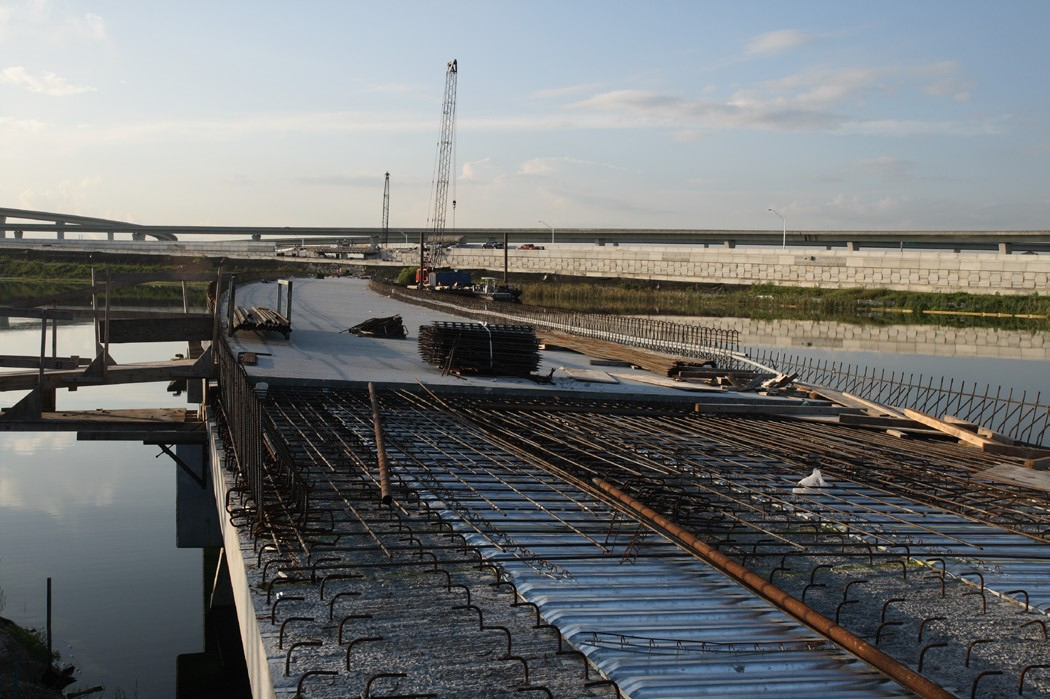
\includegraphics[width=0.7\linewidth]{cip-deck.jpg}
  % \caption{Cast-in-place concrete deck over longitudinal beams/stringers. (Courtesy Atkins North America, Inc.)}
  \caption{纵梁上的现浇混凝土桥面板}
  \label{fig:cip-deck}
\end{figure}


\subsubsection{Full-Depth Cast-in-Place Concrete Systems}

Full-depth cast-in-place concrete deck slab superstructures are a classification of bridge decks that span between pier supports without the aid of supporting beams/stringers. These deck slabs can be either solid, can contain circular voids, as shown in \cref{fig:full-depth-cip-deck}, or more trapezoidal shaped voids such as those used in cast-in-place multi-cell box structures and cast-in-place segmental structures. Voids are introduced to reduce the dead weight of the bridge. These bridge systems are usually conventionally reinforced with mild steel reinforcing, but can be posttensioned longitudinally and transversely to achieve longer span lengths.

\begin{figure}
  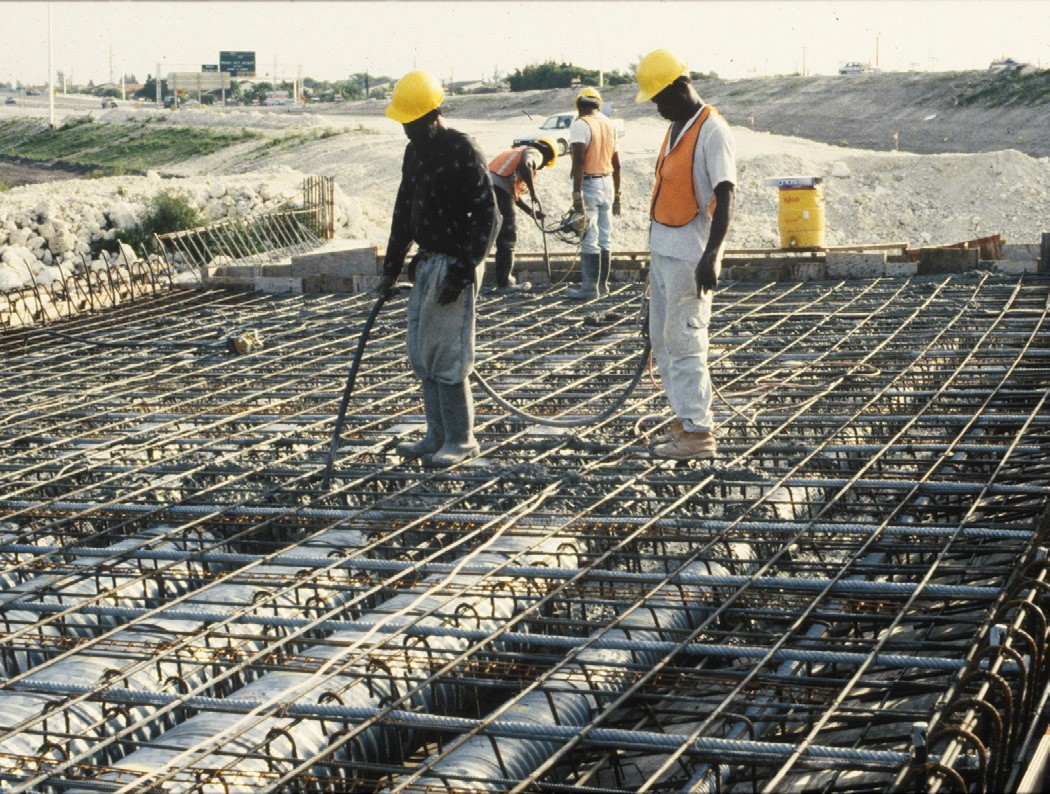
\includegraphics[height=5cm]{full-depth-cip-deck1.jpg}\hfill
  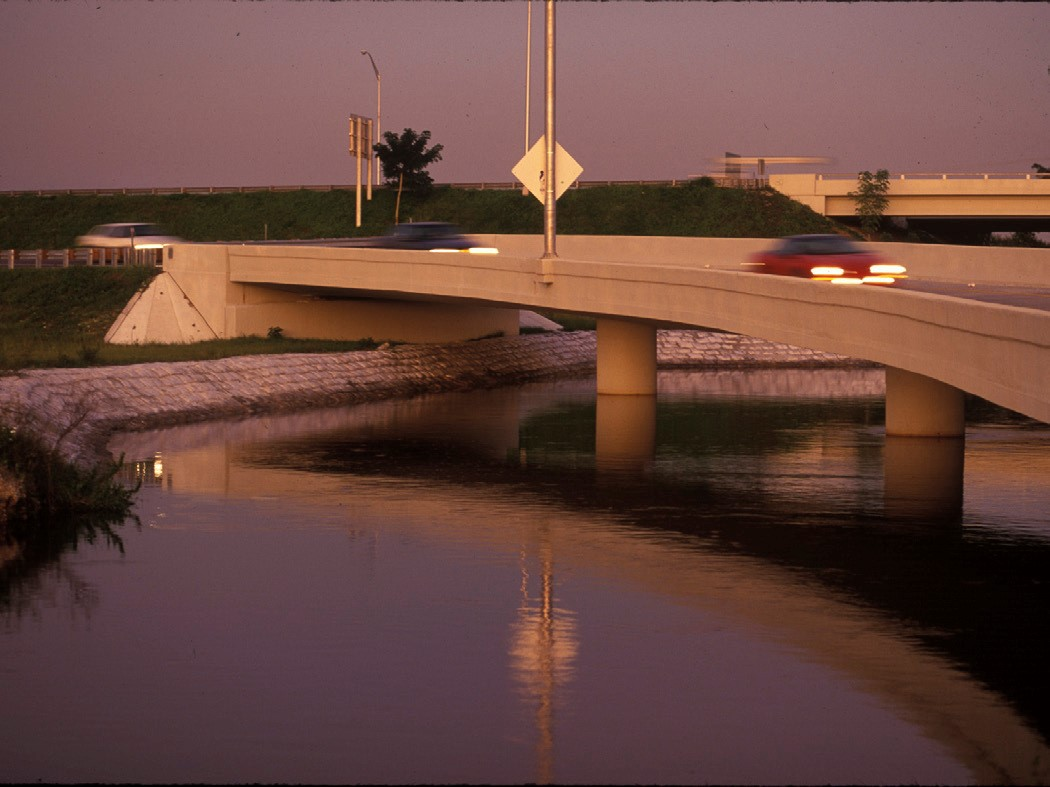
\includegraphics[height=5cm]{full-depth-cip-deck2.jpg}
  % \caption{Full depth cast-in-place concrete slab—posttensioned with voids. (Courtesy Atkins North America, Inc.)}
  \caption{全断面现浇混凝土板——间隔布置后张预应力}
  \label{fig:full-depth-cip-deck}
\end{figure}

% \subsubsection{Precast Adjacent Member Concrete Systems}
\subsubsection{Precast Adjacent Member Concrete Systems}
One of the most commonly used superstructure systems is the adjacent member superstructure system that consists of prefabricated beam elements placed side-by-side in close proximity. This system has been used in various forms to expedite construction and minimize field forming and placing of concrete. These members are predominantly prestressed concrete beam elements in the form of prestressed solid and hollow-cored slab units, as shown in \cref{fig:example-adjacent-member-slab}, deck bulb-tees, double Ts, channels and adjacent box beams. These deck systems are typically built as simple spans, but can be constructed as continuous members. Typically, the members are tied together with a continuous longitudinal grout or concrete filled shear key that allows for the transverse distribution of applied vertical forces across the joint and prevents differential movement between adjacent members. The members may also be either transversely connected with conventional reinforcement or posttensioned together to develop the moments across the joint.
% 最常用的上层建筑系统之一是相邻的成员上层建筑系统,该系统由预制的光束元素组成,并紧密接近。 该系统以各种形式使用,以加快构造并最大程度地减少混凝土的田间形成和放置。 这些成员主要是预应力的混凝土束元素,其形式是预先固体和空心式平板单元的形式,如\ cref {fig:example-adjacent-member-slab},甲板灯泡,双TS,双TS,通道和相邻盒子 梁。 这些甲板系统通常以简单的跨度构建,但可以作为连续成员构建。 通常,成员与连续的纵向灌浆或混凝土填充的剪切钥匙绑在一起,该剪切键可以使跨关节上施加的垂直力的横向分布,并防止相邻成员之间的差分运动。 成员也可以横向与常规加固相关,或者可以一起张开,以发展整个关节的力矩。

\begin{figure}
  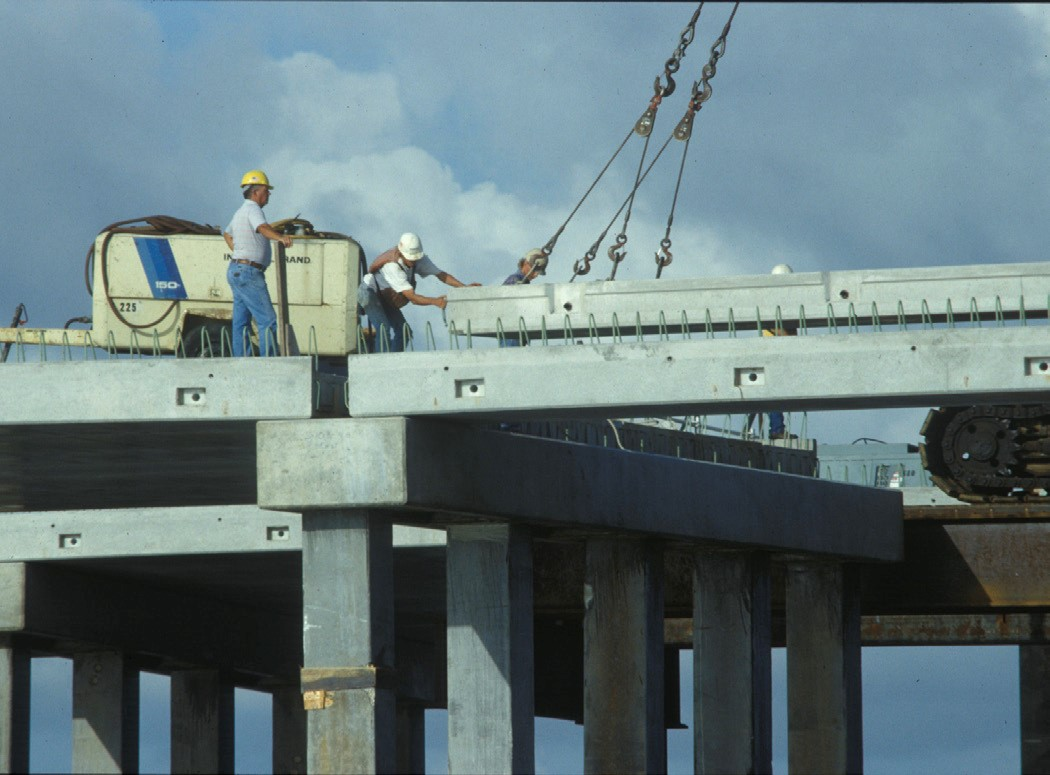
\includegraphics[width=0.7\linewidth]{example-adjacent-member-slab.jpg}
  % \caption{Examples of adjacent member slab unit superstructure system. (Courtesy Atkins North America, Inc.)}
  \caption{Examples of adjacent member slab unit superstructure system. (Courtesy Atkins North America, Inc.)}
  \label{fig:example-adjacent-member-slab}
\end{figure}

% \subsubsection{Precast Concrete Deck Panels}
\subsubsection{Precast Concrete Deck Panels}
As shown in \cref{fig:precast-panel}, precast concrete deck panel systems employ a series of precast concrete panels that are usually full-depth in thickness and have a length and width determined by specific bridge geometry. The length of the panel along the roadway is approximately 8 to 12 ft, and is typically dictated by transportation limitations and crane capacity. Panels span across the supporting girders and are designed with conventional reinforcement or as prestressed concrete. The general preference of precasters/contractors is to use prestressed concrete to eliminate possible cracking from handling and shipping.

Precast concrete deck panel systems include both transverse and longitudinal slots for connections. The transverse slots are typically grout-filled keyways connected in a manner similar to the adjacent member bridge systems. The longitudinal slots may consist of grouted (or concreted) pockets or block-outs to accommodate the shear connections to the girder. The system may also require temporary support and forms along the girder to retain the grout and some type of overlay to improve pavement ride quality. Longitudinal posttensioning is typically included in the system to tie the panels together; however, systems without posttensioning have been used and at the time of writing (2012), new non-posttensioned connections are being developed.

\begin{figure}
  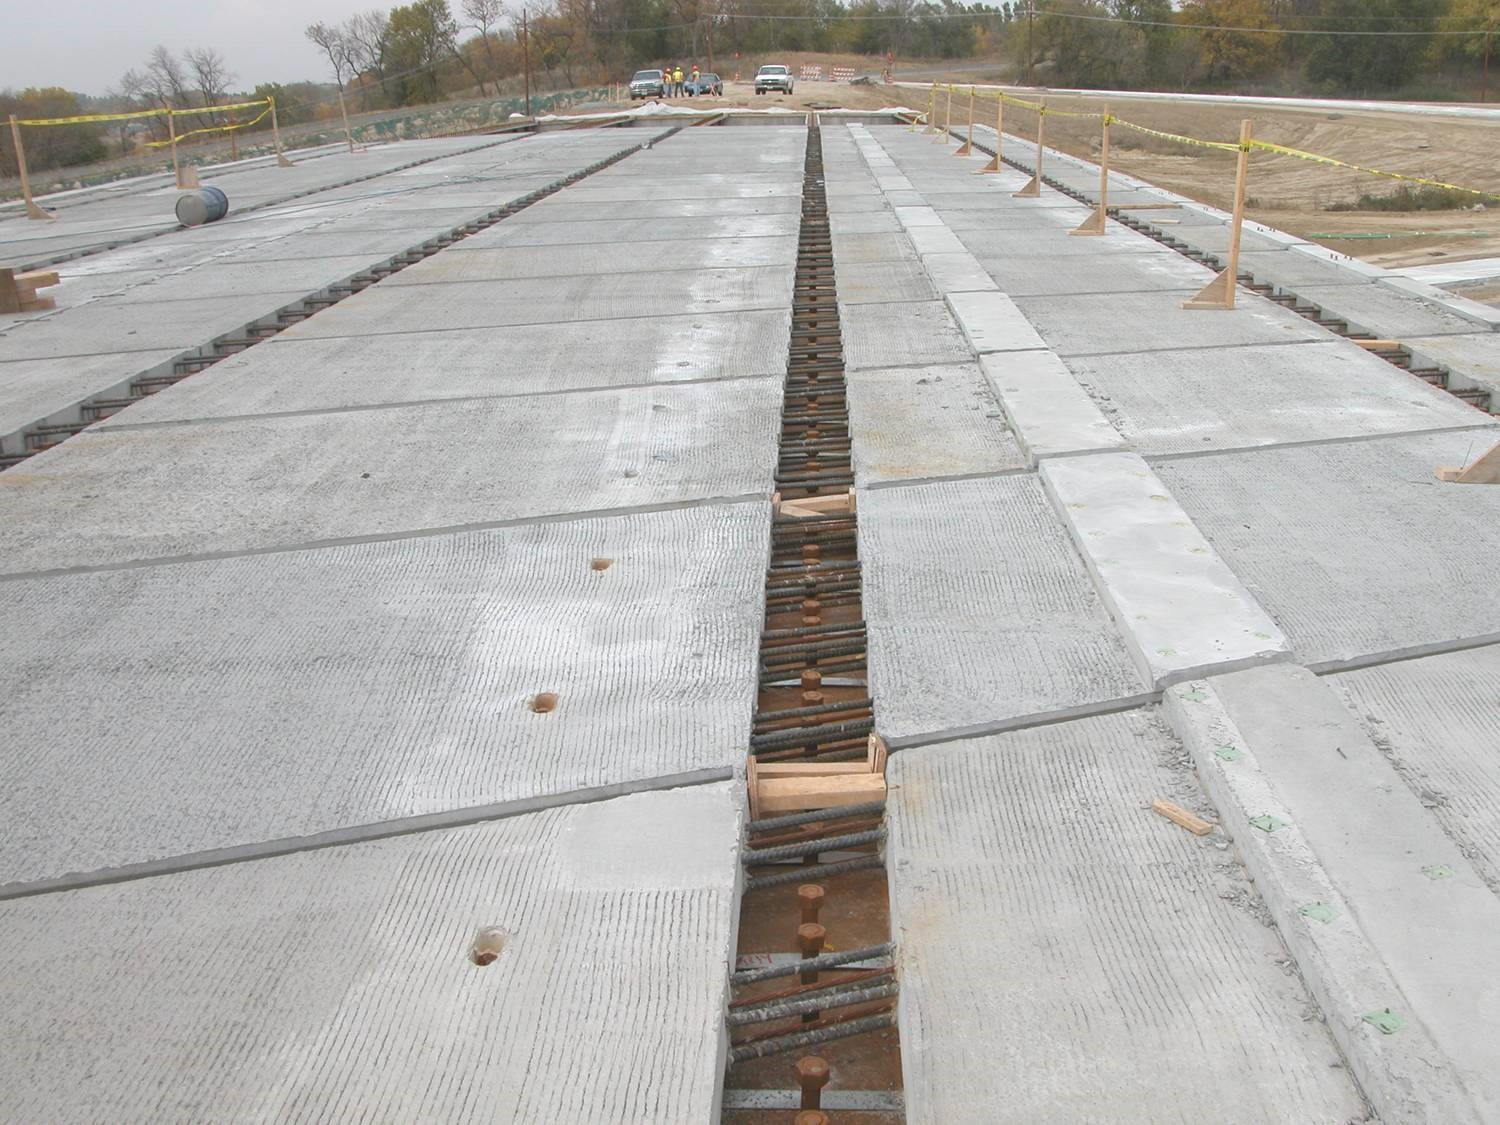
\includegraphics[width=0.7\linewidth]{precast-panel.jpg}
  % \caption{Full-depth Precast Panel System. (Courtesy University of Nebraska, Omaha)}
  \caption{全断面预制桥面板}
  \label{fig:precast-panel}
\end{figure}

% \subsubsection{Precast Segmental Concrete Superstructure Systems}
\subsubsection{预制混凝土节段拼装上部结构}
This structural system consists of numerous precast bridge elements that are posttensioned together to form either simple-span units or, more commonly, continuous spans. Segmental construction has gained favor in situations where access is challenging, such as in deep valleys, environmentally sensitive areas, across existing roadways, and where accelerated construction is warranted. The basic cross-section of a segmental bridge is usually a box shape with a top slab serving as the bridge deck-riding surface, as shown in \cref{fig:segmental-superstructure}. The primary longitudinal reinforcement consists of either posttensioning tendons or bars that can be installed either internal to the web or externally inside the box section. The bridge deck is typically posttensioned transversely.

\begin{figure}
  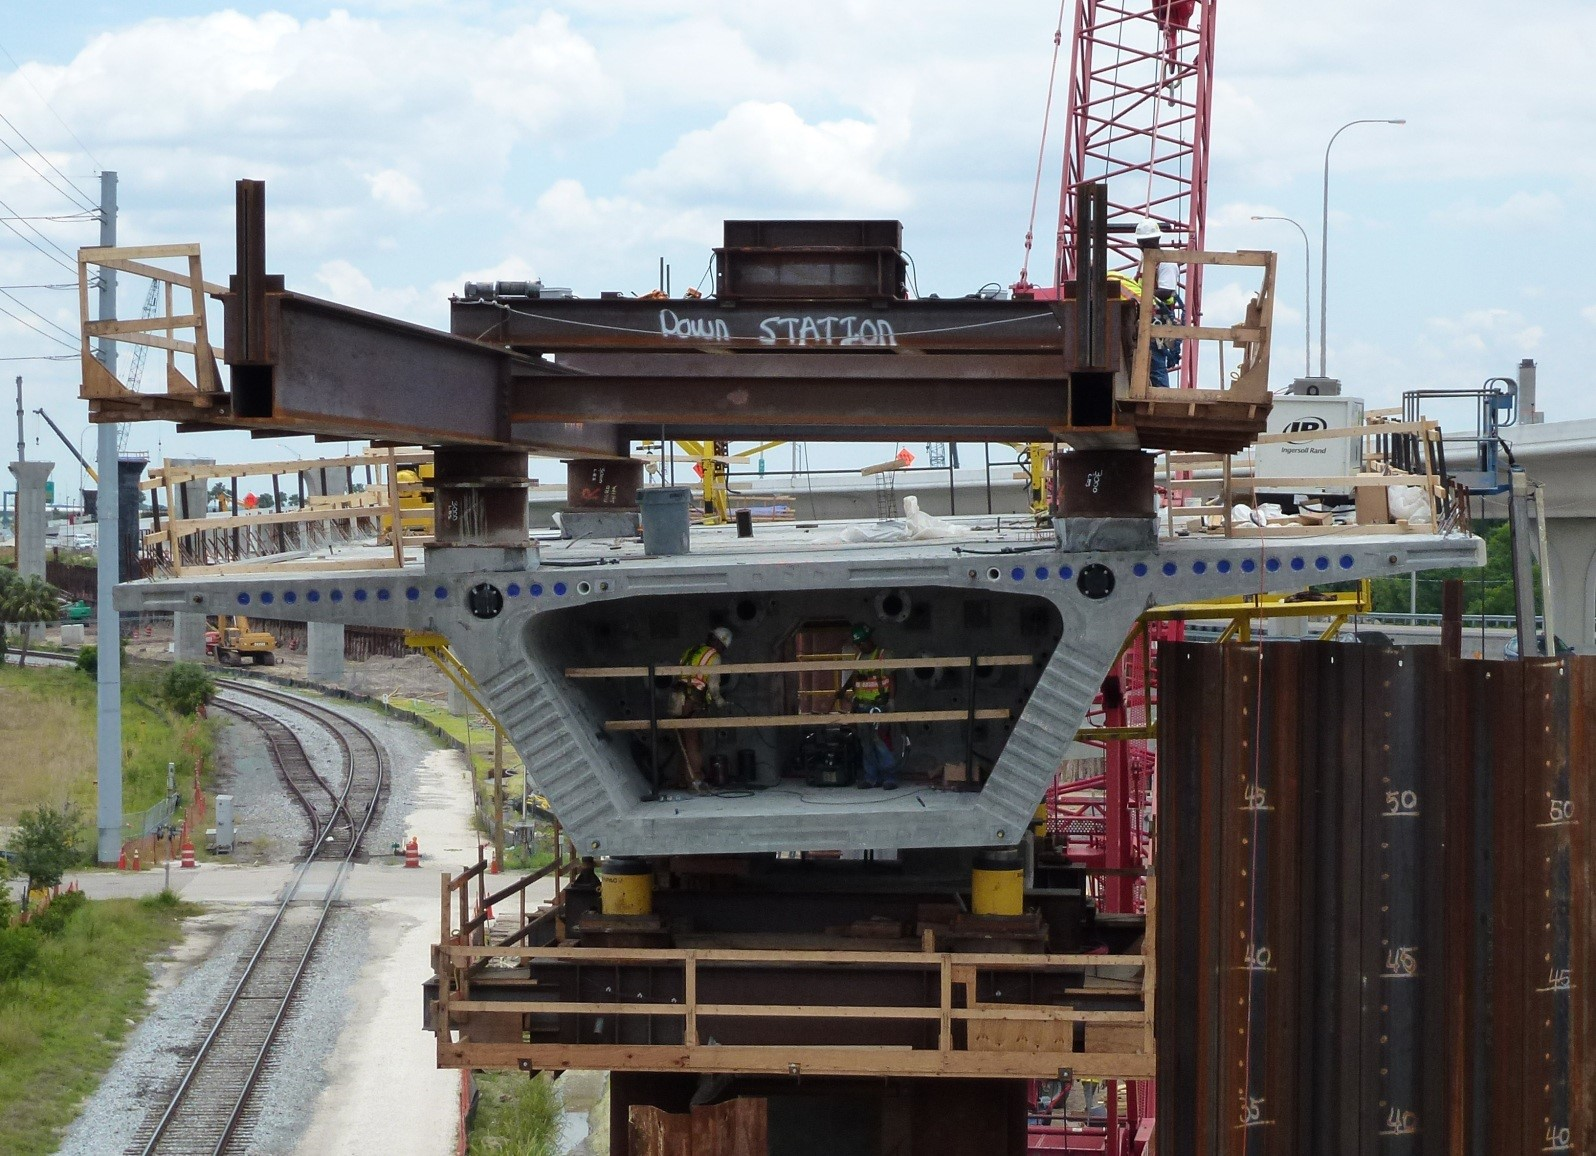
\includegraphics[width=0.7\linewidth]{segmental-superstructure.jpg}
  % \caption{Segmental superstructure. (Courtesy Atkins North America, Inc.)}
  \caption{节段拼装上部结构}
  \label{fig:segmental-superstructure}
\end{figure}

% \subsection{Metal Deck Systems}
\subsection{金属桥面系}
Metal deck systems are bridge deck systems that rely on a metal such as steel or aluminum to provide the structural resistance to vehicle wheel loads. Metal deck systems can consist of metal grid decks, orthotropic steel decks, or orthotropic aluminum decks.

% \subsubsection{Metal Grid Decks}
\subsubsection{Metal Grid Decks}
This bridge deck system is a prefabricated module system consisting of main I- or T-shaped sections and secondary crossbars combined to form a rectangular or diagonal pattern. These members can be either steel or aluminum and the main elements span between beams, stringers, or other crossbeams. This system is typically used for movable bridges and for long-span structures where a reduced bridge deck weight is demonstrated to have an economic advantage. It has also been used in deck replacement projects. The system consists of open grid deck or can be combined with concrete to form a partially or fully filled grid deck. The partially- or fully-filled concrete is typically cast flush with the grid service, or it can be cast above the unfilled deck. This is known as the Exodermic™ bridge deck system. The addition of concrete in these systems reduces noise, improves fatigue performance, and improves the ability to channelize and collect storm water.


% \subsubsection{Steel Orthotropic Decks}
\subsubsection{正交异性钢桥面板}
\label{subsubsec:steel-orthotropic-deck}
Bridge structures can utilize the orthotropic steel plate as one of the key structural systems in the distribution of deck traffic loads and for stiffening the supporting slender plate elements in compression. Generally, the orthotropic system consists of a flat, thin steel plate, stiffened by a series of closely-spaced longitudinal ribs at right angles or orthogonal to intermediate floor beams. (See \cref{fig:orthotropic-steel-deck}.) The orthotropic deck is typically made integral with the supporting bridge superstructure as a common top flange to the floor beams and girders. This results in cost savings in the design of these other components. The defining characteristic of the orthotropic steel bridge is that it results in a nearly all-steel superstructure.

\begin{figure}
  % \includegraphics[width=\linewidth]{graphic-file}
  % \caption{Orthotropic steel deck bridge. (Wolchuk 1963)}
  \caption{正交异性钢桥面板}
  \label{fig:orthotropic-steel-deck}
\end{figure}

The orthotropic system has been utilized for many bridges worldwide, especially in Europe, Asia, the Far East, and South America. The United States has not yet fully embraced this technology and currently has fewer than 100 such bridges in inventory. The orthotropic deck has been most commonly used in the United States for long-span bridges in which the minimization of dead load is paramount and for re-decking bridges on urban arterials. Orthotropic construction has tremendous potential for use in short- to medium-span girder bridges. The system has not been used more extensively for economic reasons; however, its light weight makes it beneficial for increasing a bridge’s load rating during a deck replacement in instances where replacement of the bridge may have been the only other alternative.



% \subsubsection{Aluminum Orthotropic Decks}
\subsubsection{正交异性铝桥面板}
The aluminum orthotropic deck system configuration is similar to the steel orthotropic deck described in \cref{subsubsec:steel-orthotropic-deck}. The use of aluminum provides a corrosion resistance advantage that can result in lower maintenance costs, as it does not need periodic painting. While aluminum is lighter than steel, its additional cost has often deterred its use in the United States. Other factors to carefully consider that make it different from the steel orthotropic deck system include differences in thermal expansion coefficients, reactions with dissimilar materials, lower modulus of elasticity and lower fatigue strength of the material, particularly at weld locations.


% \subsection{Timber Bridge Decks}
\subsection{Timber Bridge Decks}

Timber bridge decks have been used for hundreds of years, but increases in vehicle loads have typically restricted their use to low volume roadways. The materials used for these bridge decks can be rough sawn timbers, gluelaminated panels. Their performance can be enhanced through the use of protective coatings that can minimize water absorption, which can be detrimental to the service life of the timber.

The timbers can be posttensioned together to form stress-laminated decks, or nailed together to form spikelaminated decks. Overlays are typically provided on these bridges to improve skid resistance; however, the overlay requires extensive maintenance due to the flexibility of the timbers and the numerous connections between members.

% \subsection{Fiber Reinforced Polymer (FRP) Bridge Decks}
\subsection{\texorpdfstring{\acrlong*{frp}}{FRP}桥面板}

Fiber reinforced polymer bridge decks and superstructure systems are an emerging technology. FRP decks have been used for short-span bridges and for deck replacement on bridges. The principal advantages of FRP as a material are that it does not corrode under the same conditions as steel materials and it is lightweight. Its potential has shown promise for use in projects where deck replacement is needed, as shown in \cref{fig:frp-bridge-deck}, particularly if total load capacity is relatively low.

FRP bridge decks and superstructures have been constructed in many states. Comparisons with traditional castin- place concrete bridge deck systems have shown that they exhibit lower dead loads, higher live load fatigue ranges and lower dynamic allowance (impact). (Albers et al. 2007)

\begin{figure}
  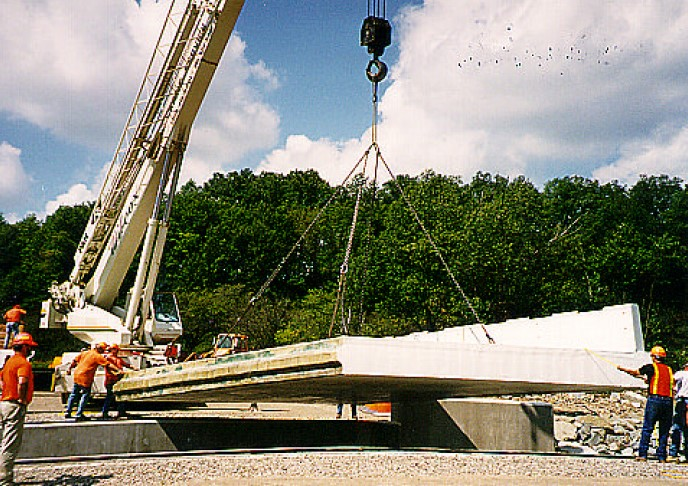
\includegraphics[height=6cm]{frp-bridge-deck1.jpg}\hfill
  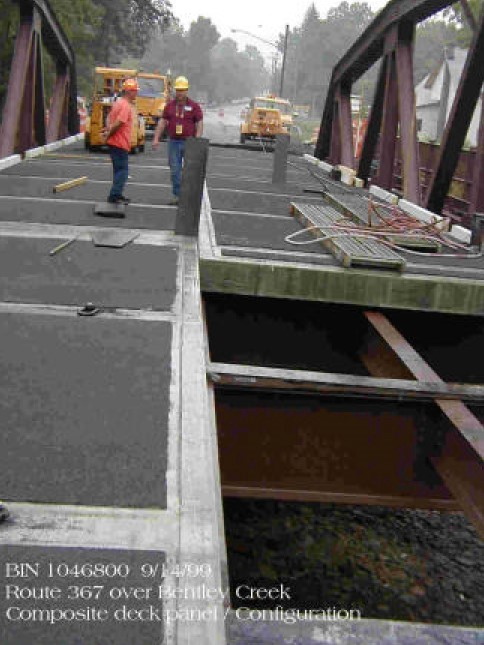
\includegraphics[height=6cm]{frp-bridge-deck2.jpg}
  % \caption{FRP bridge deck and superstructure applications. (Aboutaha 2001)}
  \caption{\acrshort*{frp}桥面板}
  \label{fig:frp-bridge-deck}
\end{figure}

The surface of the FRP material has low skid resistance and the material itself is soft. Therefore, overlay systems are required to provide a safe riding surface that has adequate surface friction, and in order to withstand daily traffic wheel load abrasion. Failure of overlay adherence to the FRP material was evidenced in early applications of this technology. Connections for crashworthy barriers for FRP decks present additional challenges.

Further research is recommended to study the long-term behavior of this new material to demonstrate its acceptability to provide a sufficiently long service life.

\section{Factors Influencing Bridge Deck Service Life}
\label{sec:factors-influence}

Bridge decks are one of the most costly maintenance items within a typical bridge system. The reduced service life of bridge decks can be attributed to two causes: 
\begin{enumerate*}
  \item obsolescence, which is a functional planning issue and not a factor relating to durability issues, and 
  \item material service life performance deficiencies, which may be load-induced, caused by man-made or natural hazards, or result from production defects in construction processes and/or design details, or operational procedures. 
\end{enumerate*}
These deficiencies are illustrated in the fault tree shown in \cref{fig:fault-tree-bridge-deck}.

\begin{figure}
  % \includegraphics[width=\linewidth]{graphic-file}
  % \caption{Bridge deck reduced service life fault tree.}
  \caption{桥面板导致\gls*{servicelife}\gls*{faulttree}}
  \label{fig:fault-tree-bridge-deck}
\end{figure}

Many interrelated factors during the design, construction, and management phases of a bridge deck’s service life must be considered in developing long-lasting, cost-effective bridge decks. These factors vary depending on the bridge deck system utilized and can be arranged in four broad categories:
\begin{itemize}
  \item Concrete bridge decks systems, including:
  \begin{itemize}
    \item Cast-in-place concrete bridge deck systems, and
    \item Precast concrete bridge deck systems;
  \end{itemize}
  \item Metal deck systems;
  \item Timber deck systems; and
  \item FRP bridge deck systems.
\end{itemize}

The factors affecting the service life of cast-in-place concrete and precast concrete bridge deck systems are further described in this chapter. Metal, timber, and FRP bridge deck systems are not addressed in the Guide.

\subsection{Cast–in–Place Concrete Bridge Decks}
Cast-in-place bridge deck systems are systems in which the concrete for the bridge deck is cast in the field as an integral part of the final superstructure. This bridge deck system is one of the most common systems used in the United States today. These decks provide a major constructability advantage in that the casting process easily molds the bridge deck to meet geometric requirements, such as skews, lane tapering, and super-elevation transitions, and to match existing locations of supporting elements that are not precisely located in accordance with the plans. The main disadvantages of these decks include the quality of concrete produced as a result of workmanship and the curing processes.

Inspections of bridge decks have revealed numerous performance issues with cast-in-place concrete including cracking, corrosion of reinforcement, spalling, delamination, and concrete deterioration evidenced by scaling, wear, and abrasion. While concrete in compression is considered a very durable construction material, tension introduced through various loading and bridge restraint conditions can result in significant tension that can exceed the material's tension strength limits, resulting in cracking. Cracking of bridge deck concrete reduces the integrity of the passivated concrete layer that surrounds the reinforcing steel, significantly reducing the encased reinforcement’s resistance to corrosion.

The following sections discuss factors affecting the service life of cast-in-place bridge deck.

\subsubsection{Load-Induced Bridge Deck Considerations}
Load-induced bridge deck deterioration can be attributed to either loads induced by the traffic, or by characteristics dependent on the overall bridge system. These load-induced factors are shown in the fault tree provided in \cref{fig:fault-tree-cip-bridge-deck}.

\begin{figure}
  % \includegraphics[width=\linewidth]{graphic-file}
  \caption{Cast-in-place bridge deck load-induced deficiency fault tree.}
  \label{fig:fault-tree-cip-bridge-deck}
\end{figure}

\paragraph{Traffic-Induced Load Considerations}
Traffic-induced loads include the effects of truck and other vehicle traffic on the riding surface of the bridge. Bridge deck loading has a degree of uncertainty that must be addressed during design of the bridge, especially when achieving long service life is an objective. Typically the service life of bridge decks will be affected by fatigue, overload, and wear and abrasion.

\subparagraph*{Fatigue}
Cast-in-place concrete deck consists of two materials—steel and concrete, both of which can fail by fatigue. Design provisions for fatigue are addressed in the LRFD Specifications.
\subparagraph*{Overload}
Despite weight limit regulations in most states that define load limits for permit and legal truck configurations, overloads exceeding these limits do occur. This is one of the main reasons for reduced service life of bridges.

Overloads result in additional flexural stresses in bridge decks that can cause excessive cracking not accommodated by the original design. Heavier tire loads may also affect the wear and abrasion on the structure, and multiple applications of these loads can affect the fatigue behavior of the deck.
\subparagraph*{Wear and Abrasion}
Wear and abrasion is typically affected by high traffic volume, high tire loads, and the types of tires used on the facility. Tires in cold climates may have enhanced features to aid in traction, such as deep grooves, studs, and chains. These added tire features, while aiding traction, can abrade the surface of the bridge deck.

Wear and abrasion can result in reduced thickness of the bridge deck, which in turn reduces the concrete cover protecting the reinforcement from corrosion; can reduce the load resisting section resulting in higher stresses and cracking; and can change the deck stiffness assumed for distribution of loads between superstructure elements.


\paragraph{System-Dependent Loads}
System-induced loads include the effects of the bridge system configuration on the behavior of the bridge deck, such as restraint of integral abutment systems.

\subparagraph*{Differential Shrinkage}
Differential shrinkage occurs when bridge deck concrete is cast over previously cured concrete or over steel girders. The shrinkage of fresh concrete is restrained by the cured concrete or steel stringers resulting in a set of equal and opposite forces causing tension in the deck and compression in the girders. Heat of hydration also contributes to development of tensile forces in the freshly cast concrete deck.
\subparagraph*{System Framing Restraint}
Bridge decks can be subject to additional axial forces created by bridge boundary conditions. Bridge system boundary conditions are set at the design stage, during bridge system selection. For instance, in integral abutment jointless bridge systems, the elimination of expansion devices and reliance on flexibility of piles to resist the bridge expansion and contraction, subject the deck to additional axial forces. Another example of boundary conditions capable of creating axial forces in bridge deck includes choices for bearings and connections between superstructure and substructure made during design. These axial forces range from compression during system expansion to tensile forces during system contraction. Resistance to system contraction can create tensile forces in the bridge deck and cause cracking. Calculation of these additional axial forces is important and can be achieved through conducting proper analysis methods that correctly model the bridge boundary conditions.

Improper function, or seizing of the bearings, results in unintended movement restraint that can raise the force resisted by the substructure well above the intended design. This unintended restraint can cause unanticipated cracking with greater potential for corrosion. Proper bearing function is essential to the durability of substructure and is addressed in \cref{chp:bridge-bearings}. Lack of maintenance may also result in bearings losing the movement capability intended by their design.

\subparagraph*{Thermal}
Temperature changes can result in the development of axial forces in the bridge deck. These thermal forces are due to uniform internal temperature changes and temperature gradient. The level of these thermally induced axial forces is a function of bridge system boundary conditions.


\subsubsection{Natural or Man-Made Hazard Bridge Deck Considerations}
The environment to which the bridge deck is subjected can have a significant influence on the service life of bridge decks. These environmental influences include hazards from both natural and man-made sources, and include effects from areas with adverse thermal climate, coastal climates, and chemical climates, as well as from chemical properties of the materials and outside agents, such as fire. These natural and man-made hazards are introduced in the fault tree provided in \cref{fig:fault-tree-cip-deck-hazard}.

\begin{figure}
  % \includegraphics[width=\linewidth]{fault-tree-cip-deck-hazard}
  \caption{Cast-in-Place Bridge Deck Natural or Man-made Hazard Fault Tree}
  \label{fig:fault-tree-cip-deck-hazard}
\end{figure}

\paragraph{Thermal Climate}
Thermal climate influences on bridge deck service life performance are primarily due to cold weather. These influences are both manmade, from the application of deicing salts, and natural, in the case of freeze/thaw.

\subparagraph*{Application of Deicing Salts}
Agencies in cold weather climates that deal with ice and snow on roadways and bridges have traditionally applied deicing salts to melt the ice and snow to facilitate tire traction. The application of these deicing salts is viewed as a safety enhancement for the traveling public; however, these chloride-laden compounds tend to ingress into the concrete deck either through porosity in the concrete or through open deck cracks. The chloride ingress into the bridge deck continues to reduce the effectiveness of the passivating layer around the reinforcing steel, eventually initiating reinforcement corrosion. The reinforcement corrosion process causes the bar to expand, resulting in deck cracking, spalling, and/or delamination. The cross-slope built into bridge decks for drainage purposes causes the salt to wash down towards the bridge gutter adjacent to the traffic railing barriers bounding the bridge. Removal equipment that scrapes snow from the bridge deck also deposits residual snow laden with deicing salts at this location, resulting in a very high concentration of chlorides. Construction joints at this location are particularly susceptible to chloride intrusion, and in many cases this has led to corrosion of the barrier reinforcement.

\subparagraph*{Freeze/Thaw}
Water absorbed into the concrete deck surface and contained in cracks can freeze in cold weather conditions. The frozen water tends to expand causing stresses within the concrete. Cyclic freezing and thawing of the water absorbed in the deck surface can result in bridge deck deterioration in the form of cracking, scaling, and spalling. Refer to \cref{chp:materials} for additional information on freeze/thaw in concrete.

\paragraph{Coastal Climate}
Coastal climate influences on bridge deck service life performance are primarily due to the introduction of
chlorides through salt spray, and from the effects of high humidity. Both of these influences occur naturally.

\subparagraph*{Salt Spray}
Coastal regions are subjected to a chloride-laden saltwater environment and a combination of wind
and wave action that causes these chlorides to become airborne as salt spray. The susceptibility of the bridge deck to
these environmental influences depends on the height of the bridge deck above the water elevation and the distance
to coastal areas. The action of waves hitting substructure units and seawalls or abutments under the bridge tends to
cause the salt spray to explode upwards, wetting the bottoms of lower level bridge decks. The salt spray can also
deposit itself on the bridge deck surface, particularly on windy days. When the salt spray wets the surfaces it leaves a
chloride residual that can absorb into the concrete, resulting in reinforcement corrosion.

\subparagraph*{Humidity.}
High humidity in coastal regions also results in cyclical wetting and drying of concrete surfaces.
Concrete materials sensitive to repeated wetting, such as those where reactive aggregates are utilized, can have an
adverse effect on the bridge deck service life.

\paragraph{Chemical Climate}
Chemical climate influences on bridge deck service life performance can be attributed to corrosion-inducing
chemicals and sulfate attack. These influences can occur naturally or can be man-made.

\subparagraph*{Corrosion-Inducing Chemicals}
Corrosion-inducing chemicals can be introduced to the bridge deck from
adjacent industries, where residuals from pollution can attribute to reduction in bridge deck service life. For example,
oil and coal burning facilities release sulfur dioxide and nitrogen oxide into the air, which causes acid rain consisting
of sulfuric and nitric acids. These acids can dissolve cement compounds in the cement paste and calcareous
aggregates, and can leave crystallized salts on concrete surfaces that can lead to spalling and the corrosion of
reinforcing bars.
\subparagraph*{Sulfate Attack}
Exposure to sulfates can cause expansion of the concrete material and consequently result in
spalling and cracking of bridge deck. Refer to \cref{chp:materials} for additional information on sulfate attack in concrete.

\paragraph{Reactive Ingredients}
Reactive ingredients within the mix used for bridge decks can affect service life performance as the reactive
ingredients alter the volumetric stability of the concrete. These influences primarily occur naturally.
\subparagraph*{Alkali-Silica Reactivity}
Alkali-silica reactivity (ASR) results in swelling within concrete that can lead to spalling, cracking, and general concrete deterioration. Refer to \cref{chp:materials}, for additional information on ASR in concrete.

\subparagraph*{Alkali-Carbonate Reactivity}
Alkali-carbonate reactivity (ACR) results in aggregate expansion within concrete that can lead to spalling, cracking, and general concrete deterioration. Refer to \cref{chp:materials} on materials, for additional information on ACR in concrete.

\paragraph{Fire}
A key factor in the amount of damage that is caused to concrete is the duration of the fire and the heat levels
generated. Because of the low thermal conductivity of concrete, it takes considerable time for the interior of concrete
to reach damaging temperatures. When concrete is exposed to the extreme heat of a fire, the chemical bonds between
the water molecules in the concrete break, resulting in dehydration and the destruction of the cement binder. The
concrete loses its mechanical properties, exhibiting cracking and spalling, and exposes steel, leaving it unprotected (ACI 216, 1989). Once the reinforcement has become exposed, it conducts heat and accelerates this action.
Reinforcing steel in bridge decks subjected to temperatures above 550°C (1022°F) exhibits a rapid reduction of
strength, which can lead to collapse. In addition, spalling can result from the rapid quenching of hot fires by fire
hoses.

\subsubsection{Design, Construction (Production), and Operation Bridge Deck Considerations}
Decisions made for the design and construction of bridge decks and the activities that will occur during its
operation can have a significant influence on the service life. These influences are introduced in the fault tree
provided in \cref{fig:fault-tree-cip-deck-operation}, and include decisions made during the design and detailing of the bridge deck, the quality of
construction, the level of inspection, and the testing performed during operations and maintenance.

\begin{figure}
  % \includegraphics[width=\linewidth]{fault-tree-cip-deck-operation}
  \caption{Cast-in-place bridge deck design, construction (production), and operation defects fault tree.}
  \label{fig:fault-tree-cip-deck-operation}
\end{figure}

\paragraph{Design and Detailing Bridge Deck Considerations}
Decisions made during the design and detailing phase of a bridge project can significantly impact the service life
of the bridge. It is incumbent upon designers to understand the implications of these decisions in order to make
rational choices that will improve the service life of bridge decks. These decisions are introduced in the fault tree
provided in \cref{fig:fault-tree-cip-deck-design}, and include choices in design philosophy, expansion joints, construction joints, concrete mix
design, and bridge deck drainage.

\begin{figure}
  % \includegraphics[width=\linewidth]{fault-tree-cip-deck-operation}
  \caption{Cast-in-place bridge deck design/detailing deficiency fault tree.}
  \label{fig:fault-tree-cip-deck-design}
\end{figure}

\subparagraph{Design Philosophy}
There are two principal methods presented in the LRFD Specifications for the design of bridge decks: the
traditional design method and the empirical design method.

\emph{Traditional Design Method}.The traditional design method assumes flexural action to describe behavior of bridge
deck spanning between supporting girders and ignores the axial forces created in the bridge deck as a result of arching action. Under this assumption, the amount of reinforcement needed in the bridge deck will generally far
exceed the demand, usually by more than a factor of two. Providing additional reinforcement in the bridge deck
creates additional means for corrosion and deterioration of bridge deck.

\emph{Empirical Design Method}. The empirical design method provides better estimation of bridge deck resistance to
applied traffic loads than the traditional design method. Test results (Fang 1985; Holowka 1980) show that the
principal mechanism for resisting the applied traffic loads in the bridge deck is the creation of axial compressive
loads, commonly referred to as arching action. These axial compressive loads are resisted by supporting longitudinal
beams. Consequently, the use of the empirical method is not applicable to cantilever portions of the deck. The axial
compressive loads in the bridge deck significantly reduce the need for reinforcement in the bridge deck and reduction
of reinforcement in the bridge deck significantly reduces the sources of corrosion.

\emph{Other Design Methods}. Research in Canada in the past 15 years (Newhook and Mufti 1996) has focused on
eliminating bridge deck reinforcement corrosion through the development of the concept of “steel-free” bridge decks.
Similar to the methodology employed by the empirical design method, this concept provides the tension tie required
to resist the compressive forces created in bridge deck by arching action. Under this concept, the tension ties are
attached to top flanges of the supporting beams/stringers. These bridges have experienced some temperature and
shrinkage cracking and in order to control this cracking to acceptable levels, recent recommendations suggest
supplementing the steel tension ties below the deck with a mat of FRP reinforcing bars (Menon and Mufti 2004).

\subparagraph{Expansion Joints}
Expansion joints are provided to relieve system framing restraints that can cause a build-up of tension stresses in the superstructure and the bridge deck. Refer to Section 4.2.1.1.2 for additional information on system framing restraints. Refer to \cref{chp:expansion-devices}, for additional information on expansion joints.

Expansion devices provide a location within the bridge deck where dirt and other deleterious material, such as de-icing salts, can collect and produce an adverse effect on the service life of bridge decks. Impact from vehicles and from snow removal equipment can cause spalling that reduces the protective concrete cover over reinforcing and/or exposes the reinforcement, which leads to the corrosion.

\subparagraph{Construction Joints}
Construction joints are surface discontinuities where successive concrete placement regions meet and they are generally specified by the designers or construction contractors. The following are some typical construction methods where construction joints are required:

\emph{Modular Construction/Adjacent Members}. Construction joints within adjacent member superstructure systems are requirements of the modular type of construction utilized for accelerate bridge construction. Typically these joints are designed to transfer shear and moment across the interface, and if not properly designed and detailed may lead to cracking along the adjacent member interface.

\emph{Phasing of Construction}
Public pressure and demand for uninterrupted traffic flow requires some bridges to be constructed using a phased construction approach. This approach is used for both the widening of existing bridges and the construction of new bridges. In the case of new construction, a portion of the new bridge is constructed (Phase 1) while the existing bridge carries the traffic. Traffic is then transferred to the new bridge (Phase 1), the existing bridge is demolished, and the new bridge is completed (Phase 2). Finally, the two phases are typically joined together using a closure pour. The phases will experience different deflections at the time of placing the closure pour and this differential deflection can result in major construction problems.

One of the characteristics of phased constructed bridges is that transverse and longitudinal cracks form near the points where Phase 1 and 2 are joined. Formation of these cracks is a well-known feature of these bridge types. Further, closure pour regions need to be water proofed to prevent deterioration of the deck in these regions as a result of chloride ingress and initiation of reinforcement corrosion. It should also be mentioned that placing additional reinforcement in the deck will not prevent formation of these cracks; it will only make the crack width smaller.

A well-constructed phase bridge can perform very satisfactorily (Azizinamini et al. 2003). Nevertheless, several
factors as described in the following need to be taken into consideration.

Composite sections experience long-term displacement because of creep and shrinkage. \cref{fig:exaggerated-differential-displacement} shows an
exaggerated difference between elevations of Phase 1 and Phase 2 for newly constructed bridges. The same
phenomenon also exists for widening projects.

\begin{figure}
  % \includegraphics[width=\linewidth]{graphic-file}
  % \caption{Exaggerated differential displacement between phases. (Azizinamini et al. 2003)}
  \caption{Exaggerated differential displacement between phases. (Azizinamini et al. 2003)}
  \label{fig:exaggerated-differential-displacement}
\end{figure}

The reason for this observed differential displacement is illustrated in \cref{fig:displacement-phase}, which shows the displacement of the Phase 1 girders due to creep and shrinkage. In about 90 days after completion of Phase 1, the girders experience maximum creep and shrinkage displacement. As shown along the horizontal axis, construction of Phase 2
starts after Phase 1 is completed. Phase 2 also experiences the creep and shrinkage displacements and depending on
the time of casting the closure pour region, differential displacement will exist between Phase 1 and Phase 2 girders.
In the case of steel bridges, this differential deflection between the two phases has resulted in major fit up problems
for the cross frame in the bay containing the closure pour. Once the closure pour region is cast, the two systems are
locked in, while Phase 2 continues to experience additional displacements that subject the deck in the closure pour
region to additional stresses.

\begin{figure}
  % \includegraphics[width=\linewidth]{graphic-file}
  % \caption{Displacement of Phase 1 and Phase 2 portion of the bridge. (Azizinamini et al. 2003)}
  \caption{Displacement of Phase 1 and Phase 2 portion of the bridge. (Azizinamini et al. 2003)}
  \label{fig:displacement-phase}
\end{figure}

When the deck elevations of the two phases do not match, the contractor may attempt to force the two separate
superstructure portions together. This practice subjects the deck in the closure pour region to additional stresses,
which are difficult to estimate and may also jeopardize the service life of deck concrete.

There is debate and conflicting beliefs among bridge engineers on conditions under which the closure pour
region should be cast. Some contractors prefer to close traffic completely until the concrete in closure pour region is
set, while others believe that vibration caused by traffic is helpful for better consolidation of concrete in the closure
pour region. Generally, traffic closure is not an option, due to public demand that the traffic interruptions be
minimized.

Another major condition that could facilitate the construction of phased bridges is the elimination of cross frames
in the bay containing the closure pour, if possible. However, the pros and cons of such action need to be investigated.

\subparagraph{Mix Design}

\cref{chp:materials} provides detailed information concerning factors which affect the service life of concrete. The
following provides a brief description of mix design factors which affect the service life of bridge decks.

\emph{Permeability} Concrete is a durable material that largely depends on its ability to resist the infiltration of water and
aggressive solutions. Concretes with high permeability provide less resistance to aggressive solutions or water
penetrating the concrete and possibly causing expansive forces due to physical (freeze/thaw) or chemical (corrosion,
ASR, sulfate attack) factors.

\emph{Passivity around Reinforcement} The loss of passivity of the outer layer of the reinforcing steel initiates a corrosion
process that deteriorates the steel. This corrosion process begins by diffusing chloride ions to the depth of the
reinforcing steel, and/or carbonation reducing the pH of the concrete to the passivating layer surrounding the
concrete.

\emph{Crack Resistance}.Mix design can affect the extent of cracking for all cast-in-place concrete bridge decks and slab
superstructures. Mixtures with high water and paste content are prone to shrinkage cracks that occur over time. The
use of large aggregate sizes and well-graded aggregates reduces the water and paste content and minimizes
shrinkage. In fresh concrete, when the rate of evaporation exceeds the rate of bleeding, plastic shrinkage occurs. Concrete with low bleed water, stiff consistency, and low water/cement ratio is prone to plastic shrinkage cracking.
Prevention of plastic shrinkage cracking depends on prompt, effective curing.

\emph{Workability}. Concrete mix designs must include good quality aggregates and appropriate admixtures to facilitate
construction. Mix designs with poor workability can cause uncontrolled field adjustments to the mix through the
addition of water in the field, resulting in higher water-cement ratios and over-vibration that can cause aggregate
segregation. Proper workability must be ensured for the integrity of the mix design to provide concrete with the
intended properties.

\emph{Creep and Shrinkage} The creep and shrinkage properties of concrete mixes can affect the service life performance of bridge decks. The adverse effects of concrete’s shrinkage characteristics have been discussed in conjunction with system-dependent loads in Section 4.2.1.1.2. High levels of creep, on the other hand, can be either beneficial or detrimental depending on the application: 
\begin{enumerate}
  \item Beneficial when differential shrinkage occurs, particularly within bridge decks. In instances of higher creep, the restraining force between the bridge deck and the supporting superstructure will reduce significantly, consequently reducing the potential for cracking. 
  \item Detrimental when the creep results in unrestrained volumetric changes that result in significant, unintended movements of the structure, such as in posttensioned structures.
\end{enumerate}


\subparagraph{Drainage}

In design, poor drainage details can result in ponding and prolonged exposure of bridge components to moisture and aggressive solutions, causing corrosion and other environmental distress. When concrete gains moisture, it expands slightly or swells. When concrete loses moisture, the concrete contracts or shrinks. As drying occurs, the portion of concrete near the surface dries and shrinks faster than the inner portion of the concrete. This results in differential moisture condition in which tensile stresses that can cause cracks may occur on the surface.

The degree of frost damage to concrete is also highly dependent on the degree of saturation. Ponding of water on
bridge decks can cause critical saturation resulting in bridge damage. High moisture is also detrimental to concrete
susceptible to alkali-silica reactivity expansion that can cause spalling and cracking.

\paragraph{Construction}
Attention to good practices during construction is crucial to the long-term durability of reinforced concrete. A
work force that is well-qualified, well-trained, and work which is well-executed increases productivity, reduces
material waste, and provides expected service life. The proper use of appropriate equipment provides better
workability by increasing efficiency, well-planned construction schedules reduce the overall cost by providing set
times for equipment rental and reducing downtime. The correct implementation of test methods ensures quality
concrete.
\subparagraph{Placement and Curing of Concrete}
Good construction practices, which ensure the proper location of reinforcing steel for proper cover depth,
consolidation, and curing, are essential for longevity. Proper consolidation minimizes entrapped air voids that can
reduce strength and durability.

Proper curing is necessary for formation of the binder and control of volumetric changes and includes both
moisture and temperature control. In bridge structures, the deck surfaces require special attention due to their large
surface areas where loss of moisture is a concern.

Handling of concrete affects the final product. Delay in placement, particularly on hot days, should be avoided as
it can lead to stiffening of the concrete that can cause tearing of the deck surface during finishing, resulting in a poor
surface finish and reduced durability.

\subparagraph{Formwork}
The type of concrete formwork can affect the surface finish of the concrete. Impermeable forms can allow
surface voids to occur resulting in increased surface permeability, reduced strength, and an overall decrease in
durability.

Cast-in-place bridge decks on beams/stringers are cast on forms that span between the beams/stringers. These forms can be either removable or stay-in-place. Stay-in-place forms are typically made of galvanized steel, as shown in \cref{fig:cip-deck}, precast concrete panels (either conventionally reinforced or prestressed), and FRP. Many owners do not allow the use of stay-in-place forms, citing the inability to inspect the bottom surface of the concrete deck and the potential for the collection of water intruding through the cracks.

The use of precast concrete stay-in-place panels designed to be composite or noncomposite with the deck pour above, has resulted in reflective cracking over the panel joints in past applications, and has raised questions about their long-term durability. Research is needed to develop acceptable details for control or elimination of reflective cracks.

\subparagraph{System Vibration during Construction}
Excessive traffic-induced vibrations during construction can occur during the widening of a new bridge deck
that is being cast against existing bridge deck subjected to active traffic. The effect of these vibrations on the quality
of finished deck, especially in the closure pour regions, is not well understood and requires further investigation.

\subparagraph{Casting Schedule}
The casting schedule for bridge decks should carefully consider weather conditions, particularly hot days. The
rise of heat from hydration in concrete can be exacerbated by a concurrent rise in the ambient temperature, resulting
in a greater cooling differential that can cause bridge deck cracks. It takes approximately 18 hours for heat of
hydration to reach its peak value. Following casting, the concrete at the surface is always at ambient temperature,
while within the deck, the temperature varies due to the development of heat of hydration. The center of deck cools
last. As a result, the maximum temperature differential takes place between the center of the deck and the deck
surface. When the maximum temperature differential exceeds a certain limit, which most DOTs limit to about 30°F,
the deck can crack. Therefore, this maximum temperature differential needs to be controlled. When casting is
performed at night, the peak ambient temperature generally occurs 12 to 18 hours later, while the center of the deck
is at its highest temperature. This results in a minimum temperature differential that can be achieved between the
center and outside surfaces of deck concrete. On the other hand, when the deck is cast in the morning, the
temperature differential between the center of the deck and the surface of deck is much higher. In conclusion,
although casting deck at night is ideal, the common practice is to cast the concrete deck in the morning, the most
undesirable time.

\subparagraph{Casting Sequence}
Construction joints within bridge decks control the sequence of casting bridge decks, due either to concrete
volume placement constraints, or, in the case of continuous steel girders, in order to minimize bridge deck tension in the negative moment area over substructure elements. These locations form a discontinuity that can open as cracks
within the bridge deck allow ingress of moisture.


\paragraph{Visual Inspection}
Although inspections are valuable tools for identifying deficiencies in bridge decks they are typically visual,
making them subject to the ability, training, and disposition of the individual inspector. Often a deficiency is not
easily detectable and may show only subtle signs that can easily be missed by cursory inspections or by
inexperienced inspectors. Deficiencies can also be located below the undamaged surface or in inaccessible areas. The
inability to see the deficiency leads to inadequate identification of repair methods, scope, and material selection and
could cause failure of the structure without visible signs, since surficial repairs may cover the damaged area.

\paragraph{Maintenance}
Lack of preventive maintenance reduces the service life of bridge decks. Sometimes simple maintenance tasks
are delayed until a problem becomes a safety issue, at which time the required repairs may be either significantly
more extensive or ultimately irreparable.


\subsection{Precast Concrete Bridge Deck Systems}
Precast concrete bridge deck systems are systems in which the concrete components for the bridge deck are
produced in a more controlled environment, minimizing variability in concrete uniformity of both material behavior
and construction personnel performance. Use of these systems can minimize traffic disruption caused by prolonged
concrete casting operations over active roadway facilities and is a key consideration for accelerated bridge
construction.

Inspections of precast concrete bridge decks have revealed many of the same performance issues experienced
with cast-in-place concrete as described in Section 4.2.1 including cracking, corrosion of reinforcement, spalling,
delamination, and concrete deterioration evidenced by scaling, wear, and abrasion. Precast concrete bridge deck
components introduce numerous joints in the superstructure that are usually the source of many bridge deck service
life issues, particularly in cases where the material provided to seal these construction joints breaks down causing
cracking, leakage, and eventually reinforcement corrosion.

Rather than repeat the discussion of the many performance-related service life issues inherent with concrete
systems described in Section 4.2.1, this section describes the factors affecting service life specific only to precast
concrete bridge deck systems. The user of this Guide should also become familiar with the other factors described in
Section 4.2.1 when considering precast concrete bridge deck systems.

Load-induced (Section 4.2.1.1) and natural or man-made hazard (Section 4.2.1.2) bridge deck considerations for
precast bridge deck systems are the same as those for cast-in-place bridge deck systems. The following sections
discuss the factors affecting precast concrete bridge deck service life in production and operation.

\subsubsection{Design, Construction (Production), and Operation Bridge Deck Considerations}
Decisions regarding the production of bridge decks and the activities which will occur during its operation can
have a significant influence on service life. These production and operation influences are introduced in the fault tree
provided in \cref{fig:fault-tree-precast-deck-operation}. They include decisions made during the design and detailing of the bridge deck, fabrication
and manufacturing requirement, quality of construction, and decisions concerning the level of inspection and testing
performed during future operation and maintenance.

\begin{figure}
  % \includegraphics[width=\linewidth]{fault-tree-precast-deck-design}
  \caption{Precast concrete bridge deck design, construction (production) and operation defects fault tree.}
  \label{fig:fault-tree-precast-deck-operation}
\end{figure}

\paragraph{Design and Detailing Bridge Deck Considerations}
Decisions made during the design and detailing phase of a bridge project can significantly influence the service
life of the precast bridge deck. It is incumbent upon designers to understand the implications of these decisions in
order to help make rational choices that will improve service life. These influences are introduced in the fault tree
provided in \cref{fig:fault-tree-precast-deck-design}, and include choices in regard to design philosophy, expansion joints, construction joints,
concrete mix design, and bridge deck drainage. Again, many of these influences are similar to those for a cast-inplace
concrete deck, except for the addition of composite action considerations for precast decks.

\begin{figure}
  % \includegraphics[width=\linewidth]{graphic-file}
  \caption{Precast concrete bridge deck design/detailing deficiency fault tree.}\label{fig:fault-tree-precast-deck-design}
\end{figure}

\subparagraph*{Composite Action}
For precast systems such as full-depth deck panels, the design philosophy addresses either a composite or a noncomposite
connection of the deck panels to the supporting superstructure element.

\emph{Composite systems} Composite bridge deck systems add to the stiffness of the overall bridge system, reducing deflection and vibration and improving bridge deck performance. The connection requirements for composite systems are developed through field casting of concrete or grout around shear connectors or studs accessed through continuous full depth open pockets as shown in \cref{fig:precast-panel}, through localized, full-depth open pockets, or through continuous or localized embedded channels in the panels under the deck surface. Open pocket systems introduce construction joints, forming a discontinuity that can open as cracks. Embedded channel systems require pressure grouting to fill the void. Improper grout installation can lead to entrapped air voids that can fill with bleed water and water intruding through deck cracks, leading to freeze/thaw issues and increased potential for reinforcement corrosion.

\emph{Non-composite systems}
In non-composite systems, excessive flexibility and inconsistent friction between the deck
panels and the superstructure along the length of the supporting stringer could result in localized stress that can cause
cracking and delamination in the concrete. Excessive vibrations can also lead to fatigue issues.

\paragraph{Modular Joint Construction}
In precast systems consisting of adjacent members or segmental construction, the design and detailing of the joint
is essential to its proper performance. These joints can open as cracks within the bridge deck if not properly
considered, leading to leakage, spalling, and reinforcement corrosion.


\paragraph{Precast Component Fabrication and Manufacturing Considerations}
Decisions relating to the fabrication and manufacturing of precast components for bridge decks can significantly impact the service life of the bridge. It is incumbent upon the fabricators to understand the implications of these decisions in order to help make rational choices for improving the service life of bridge decks. These decisions are introduced in the fault tree provided in \cref{fig:fault-tree-precast-deck-operation}, and include choices in field fit-up and casting tolerances, as well as methods for lifting the precast elements in the precast yard and for erection in the field.

\subparagraph{Tolerances and Field Fit-Up}
Careful planning must be utilized to incorporate precast components as bridge decks on bridges. These components must be aligned in the field fairly accurately to ensure a smooth, safe ride for the travelling public. Often the construction sequence and schedule must be assessed to establish casting dimensions for the precast components. Liberal tolerances and insufficient control in the precasting facility can result in ill-fitting pieces that require unintended adjustments in the field leading to spalling and other structural failures due to localized, non-uniform contact surfaces that were not anticipated during design.

\subparagraph{Transportation and Lifting Methods}
Precast components must be moved from the casting facility to their final position in the bridge, a transport that may consist of multiple lifts depending on storage requirements and transportation schedules. These components must also be transported between the casting bed, storage facilities, and the project site. Improper consideration of the stresses imposed on the precast component during these critical events can result in cracking, spalling, and sometimes failure.

Lifting precast components also requires devices for attaching slings and/or cables, usually consisting of steel
embedded in the finished surface of the concrete. Improper removal and treatment of these embedments once the
precast component is set in the field can result in localized spalls due to steel corrosion.

\paragraph{Construction}
Attention to good practices during construction is crucial to the long-term service life of reinforced concrete. Well-qualified, well-trained, and well-executed workmanship increases productivity, reduces material waste, and provides expected service life. Proper use of adequate equipment provides better workability by increasing efficiency, and a well-planned construction schedule reduces the overall cost of the project by providing set times for equipment rental and reducing downtime. Proper use of test methods is needed to ensure that quality concrete is achieved. These practices are introduced in the fault tree provided in \cref{fig:fault-tree-precast-deck-operation}, and include workmanship related to the connectivity of the precast components.

Connection of precast components is performed in several ways. Match cast components are typically joined with epoxy and prestressed across the joint. Improper epoxy material for the temperature of application, inadequate epoxy set time, and inconsistent, non-uniform application can cause spalling of the joint as the prestressing compresses the joint across a non-uniform contact surface.

Components that are not match cast are typically detailed with open joints to be filled with concrete or grout. Improper surface preparation and incomplete filling of these joints can result in early breakdown of the joint filler material, resulting in cracks, leakage, reinforcement corrosion, and a reduction in load distribution characteristics that can be detrimental to the carrying capacity of the bridge.

% \section{Individual Strategies to Mitigate Factors Affecting Service Life}
\section{减轻影响\glsentrytext{servicelife}因素的个别策略}
\label{sec:individual-strategy}
\cref{sec:factors-influence} defined numerous factors affecting the service life of bridge decks. This section provides individual strategies to mitigate those factors and improve service life of bridge decks. \cref{tab:mitigation-categories} summarizes the areas in which strategies are provided.

\begin{table}
  \caption{Mitigation Categories}
  \label{tab:mitigation-categories}
  \begin{tblr}{
  colspec={X[c] X[3,l] },
  row{1}={m,c,bg=genfg,fg=white,font=\bfseries,guard}
}
节 & 缓解策略 \\ 
\cref{subsec:strategies-mitigate-load-induced}     & 减轻荷载引起的效果的策略 \\ 
\cref{subsec:strategies-mitigate-system-dependent} & 减轻系统相关荷载的策略 \\ 
\cref{subsec:strategies-mitigate-hazard}           & 减轻自然或人造环境劣化的策略 \\ 
\cref{subsec:strategies-improve-operation}         & 改善制造和运营的策略 \\ 
\end{tblr}

\end{table}

% \subsection{Strategies to Mitigate Load-Induced Effects}
\subsection{Strategies to Mitigate Load-Induced Effects}
\label{subsec:strategies-mitigate-load-induced}
This section addresses concrete bridge decks. Load-induced effects are created from the traffic using the bridge and from system dependent framing restraints. Strategies for mitigating deterioration from these effects are provided in the following.

\subsubsection*{Strategies to Mitigate Traffic-Induced Loads}
A complete understanding of the traffic characteristics utilized on the structure is required to define the strategies
required for enhancing the service life of bridge decks. These characteristics include vehicle configuration, such as
axle and wheel spacing and individual wheel weights; type of wheel or tire; potential for overloads; type of
suspension system; traffic volumes and frequency of truck and overload application; and vehicle location on the
deck.

In order to establish criteria to adequately address fatigue response, overload, wear, and abrasion, these
characteristics must be understood. Table 4.3 identifies the strategies for these service life issues.

\begin{table}
  \caption{Traffic-Induced Load Mitigating Strategies}
  \label{tab:traffic-induced-strategy}
  % \input{tables/traffic-induced-strategy}
\end{table}

Bridge deck systems can be adequately designed for fatigue based on individual wheel loads, dynamic impact
considerations, and the frequency of load application developed from the volume of truck traffic to which the bridge
deck will be subjected. The fatigue design of reinforcing steel within the concrete deck is adequately addressed by
the threshold design methods provided in the LRFD Specifications.

Bridge decks can also be designed for overload conditions with adequate determination of the potential for
overload and the frequency of its application. Strategies for addressing the additional strength requirements for
overloads can be addressed by increasing the thickness of the deck.

Additional information on wear and abrasion can be found in \cref{chp:materials}. Membranes and overlays can be utilized
to separate the wheel contact surface from the deck surface.

% \subsection{Strategies to Mitigate System-Dependent Loads}
\subsection{Strategies to Mitigate System-Dependent Loads}
\label{subsec:strategies-mitigate-system-dependent}

Bridge deck performance can be enhanced by the proper selection of a system to accommodate bridge
movements, whether caused by differential shrinkage or from system framing restraints of movements from thermal
expansion and contraction, and creep and shrinkage. Table 4.4 identifies the strategies for these service life issues.


\begin{table}
  \caption{System-Dependent Load-Mitigating Strategies}
  \label{tab:system-dependent-strategy}
  % \input{tables/system-dependent-strategy}
\end{table}

These strategies are further expanded in the following sections.

\subsubsection{Differential Shrinkage}
Several enhancements are viable for addressing the restraint forces at the interface of the bridge deck and
supporting beam/stringer superstructure elements. Potential enhancements include:
\begin{itemize}
  \item Using low modulus concrete mix design, which allows the deck to accommodate the shrinkage strain with
  less tension force, which can reduce cracking. Refer to \cref{chp:materials} for additional discussion of low modulus
  concrete mix designs.
  \item Using a high creep concrete mix in the supporting superstructure element, which continues to reduce the
  locked-in tension force in the bridge. Refer to \cref{chp:materials} for additional discussion of high creep concrete mix
  designs.
  \item Using delayed composite action systems where the interface of the bridge deck and the supporting
  beam/stringer superstructure elements is not made composite until a majority of the deck shrinkage has
  occurred.
\end{itemize}

\subsubsection{System Framing Restraint}
Superstructure and substructure systems must be designed to provide either movement or restraint of the structure, with proper consideration of internally-induced forces. For additional information on the proper system
selection, see \cref{chp:bridge-system-selection} - System Selection.

\paragraph{Fully-Integral Deck Systems}
Eliminating expansion joints at abutments and over piers can enhance bridge deck performance. This bridge system is commonly referred to as a jointless bridge, and is addressed in \cref{chp:jointless-bridge}.

\paragraph{Semi-Integral Deck Systems}
A significant number of states utilize a semi-integral approach to bridge deck systems. This system provides
expansion joints at the beginning and end bridge abutments, and no joints (or limited joints) in the remainder of the
bridge. Bridge deck performance is improved by eliminating joints. Separating the bridge deck from substructure at
the abutment locations reduces the tensile forces that could otherwise be generated in the bridge deck during deck
contraction, as a result of traffic and thermal loads.


% \subsection{Strategies to Mitigate Natural or Man-Made Environment Deterioration}
\subsection{Strategies to Mitigate Natural or Man-Made Environment Deterioration}
\label{subsec:strategies-mitigate-hazard}
Proper studies for identifying environmental exposures detrimental to bridge deck performance should be
performed. Understanding of the causes of deterioration leads to proper consideration during design.

The following tables describe the strategies developed for natural and man-made environment deterioration.

\begin{table}
  \caption{Thermal Climate Environmental Deterioration.}
  \label{tab:thermal-climate-deterioration}
  % \input{tables/thermal-climate-deterioration}
\end{table}

\begin{table}
  \caption{Technology Tables for Coastal Climate Environmental Deterioration}
  \label{tab:Coastal-climate-deterioration}
  % \input{tables/Coastal-climate-deterioration}
\end{table}

\begin{table}
  \caption{Chemical Climate, Reactive Ingredient, and Fire Deterioration}
  \label{tab:chemical-climate-deterioration}
  % \input{tables/chemical-climate-deterioration}
\end{table}

Tables 4.4 through 4.7 present strategies for addressing the various factors affecting service life presented in
Section 4.2. Proper incorporation of design features and materials is important for enhancing the service life of castin-
place and precast bridge decks. Likewise, there are numerous protection strategies for enhancing the service life of
concrete bridge decks. These include providing adequate concrete cover, proper concrete mix design, proper
reinforcement selection and protection, proper drainage, application of prestressing, and the use of external protection
systems. These enhancement strategies are described in the following.

\subsubsection{Concrete Cover}
Concrete cover is recognized as an effective method for protecting steel from corrosion. A minimum top concrete
cover of two inches is required by LRFD Specifications. Generally, 2.5 in. of cover is used to allow for .5 in. of wear over the life of the deck. Cracking of the deck, however, can allow chlorides to quickly penetrate to the level of the
reinforcement, initiating the corrosion process.

\subsubsection{Concrete Mix Design}
The impermeability of concrete enhances the protection of bridge deck reinforcement. Concrete mix design is
addressed earlier in this section and is further discussed in \cref{chp:materials}.

Enhanced service life of bridge decks can be achieved by implementing a mix design to obtain desirable
properties for mitigating the potential for deficiencies. The desirable properties for enhanced performance include
crack resistance through improved tension capacity, low permeability to delay chloride intrusion, low modulus of
elasticity to allow deck strain with lower tension force, and high creep to allow reduce locked-in stresses over time.

Bridge deck concrete can also be enhanced by incorporating proper materials and admixtures, among them:
\begin{itemize}
  \item Proper cement selection. In areas where sulfate attack may be a concern, Type II or Type V cements may be
  utilized to provide added resistance to its detrimental effects. Heat of hydration, which adds to the
  differential shrinkage strain, may be reduced by using a Type IV cement.
  \item Proper aggregate selection. Some readily available aggregates may be reactive to the internal concrete
  chemistry and be more susceptible to ASR and ACR. Admixtures and/or proper blending with non-reactive
  aggregate can minimize these effects. Using high quality aggregates also enhances abrasion resistance.
  \item Proper air entrainment agent. Air entrainment increases workability in the field and also enhances concrete
  performance when subjected to freeze/thaw cycles.
  \item Proper admixture selection. Numerous admixtures are available to enhance the properties of concrete and
  improve concrete durability substantially. In particular, admixtures for concrete decks can inhibit corrosion,
  improve workability providing a proper durable concrete finish, delay initial set to provide time for concrete
  placement and finishing, and reduce water requirements to improve concrete strength and density.
\end{itemize}

It should be noted that some of these enhancements may conflict, and therefore a mix design must incorporate
desired features with the understanding that all enhancement strategies cannot be achieved. For more information on
mix designs, refer to \cref{chp:materials}.

\subsubsection{Reinforcement Selection}
The selection of bridge deck reinforcement can enhance the service life of the bridge deck and increase resistance
from corrosion and section loss, particularly in marine environments or in areas where deicing salts are used.
Enhanced reinforcing steel includes:
\begin{itemize}
  \item Corrosion-resistant reinforcing, such as FRP, stainless steel, and titanium bars;
  \item Reinforcement protection systems, such as epoxy coating and galvanizing; and
  \item Multiple posttensioning protection strategies, such as those defined by FHWA in the Posttensioning Tendon
  Installation and Grouting Manual (Corven and Moreton 2004).
\end{itemize}

Refer to \cref{chp:materials}, for more information on reinforcing materials.

\subsubsection{Bridge Deck Drainage}
Eliminating prolonged exposure to moisture, allowing the bridge deck to be maintained in a dry condition, can enhance the performance of bridge decks. Proper deck slopes, both transversely and longitudinally, should be provided to channel water to appropriate collection points. Construction joints at these collection points, as shown on the left in \cref{fig:joint-barrier}, should be eliminated or moved away from the collection point, as shown on the right in \cref{fig:joint-barrier}, to minimize contaminant intrusion, which can lead to the deterioration of reinforcement. Bridge drains, drain grates, and piping should be sized appropriately to be self-flushing, minimizing maintenance requirements.

\begin{figure}
  % \includegraphics[width=\linewidth]{graphic-file}
  \caption{Construction joint at barrier—bridge deck interface.}
  \label{fig:joint-barrier}
\end{figure}

\subsubsection{Application of Compression to Relieve Tension}
The elimination of tension in a cast-in-place bridge deck enhances the performance of the bridge deck by
eliminating or significantly reducing deck cracking. Compression is typically introduced by posttensioning the
concrete; however, the durability of the posttensioning is contingent on the proper incorporation of durability
enhancements as well. Refer to \cref{chp:materials} for additional information on the durability concerns of posttension
systems.

Compression can also be introduced into the bridge deck of continuous girder bridge systems through the use of a self-stressing bridge deck system developed by SHRP 2 R19A Project (Silva 2011). The compression in this system, typically applicable to a two-span steel girder bridge unit, is introduced by casting the bridge deck with the intermediate support higher than required. After the deck has cured, the intermediate support is lowered to its final position, thereby introducing compression into the area of the deck usually subjected to tension forces from negative moments. The system, however, requires additional research in order to establish a history of satisfactory performance. Refer to \cref{chp:provisions-self-stressing-system} for more information on this system.

\subsubsection{Membranes}
Membranes are placed on top of the concrete and are protected by an asphalt layer that also functions as a riding surface. Effective waterproofing enhances service life of the membrane system, and in turn, the bridge deck.

\subsubsection{Overlays}
The purpose of concrete overlays is to create a low permeability protective layer over the conventional concrete on bridge decks. An overlay serves as a barrier to chloride ions, therefore increasing the time required for the concentration of the ions at the level of the reinforcement to reach the threshold for corrosion. Low permeability overlays also decrease water penetration into a structure allowing it to dry out, which reduces chloride ion mobility. Overlays can be applied to new decks, or as a rehabilitation method to existing decks. However, overlays are not as effective when applied to existing decks because if chloride ions are already present in the deck when the overlay is placed, then the only protection that the overlay can offer is a decrease in moisture infiltration.

The most common type of overlay has been a low-slump dense concrete overlay, which has been effective in extending the service-life of damaged bridge decks in some states. It requires special equipment to handle the very stiff concrete, special attention to placement and consolidation are needed, and the overlays are prone to rapid loss of moisture necessitating extra care in curing. Recently, silica-fume concrete and latex-modified concrete overlays have
been successfully used in extending the service life of contaminated structures and have improved workability
compared to low-slump concrete overlays. Polymer concrete overlays are also available, generally as a temporary
repair method on damaged bridge decks. Refer to \cref{chp:materials}, Materials, for more information on overlays.

\subsubsection{Sealers}
Sealers are expected to minimize the intrusion of aggressive solutions into concrete. The primary purposes of
sealers are to prevent water and chloride ions from penetrating the concrete and thereby reduce the corrosion of
reinforcement or the deterioration of concrete.

An important property of a sealer is its vapor transmission characteristics. Moisture within the concrete needs to
pass through the sealer and escape in order to prevent high vapor pressures from building up in the concrete during
drying periods, which could cause the sealer to blister and peel.

Sealers can be either pore blockers or water repellents. Pore blocker sealers work by forming a microscopically
thin (up to 2 mm) impermeable layer on the concrete surface. Most are not appropriate for use on bridge decks
because they do not offer good skid resistance and do not hold up under traffic wear. Water repellent sealers, on the
other hand, work by penetrating slightly into the concrete and acting as hydrophobic agents. Hydrophobic sealers for
bridge decks include silanes and siloxanes.

Sealers can protect all of the exposed concrete surfaces of the structure, including bridge decks, superstructure
members, substructure members, and deck undersides. Proper surface preparation and consideration of application
rates are key factors to be considered during installation of the sealer. Abrasion, sunlight, and the environment can
affect the effective life of sealers, and resealing of the bridge deck could be expected every two to five years.


\subsubsection{External Protection Systems}
Several external protection systems are available to enhance the service life of cast-in-place bridge decks,
including electrochemical chloride extraction and cathodic protection systems.

\begin{itemize}
  \item Electrochemical chloride extraction (ECE). This system involves the application of a direct current to an
  existing bridge deck for a four to eight-week period. ECE extracts chlorides from concrete and enhances the passivated zone around the reinforcement. An anode is provided by a titanium mesh or steel anode, which is
  temporarily placed on the concrete cover. This removes an average of 40\% to 90\% of the initial free
  chlorides. The extraction depends on the depth and location of the reinforcement. The pH of the concrete is
  increased, and the remaining chloride contents are typically below threshold levels near the reinforcement
  and increase with distance from the rebar. Prior application of this technology has resulted in more than 20
  years of a passive/non-corroding condition. Typically applied to existing bridge decks, this system also has
  potential to pre-treat a new concrete bridge deck, enhancing the passivated zone around the reinforcement.
  \item Cathodic Protection. Cathodic protection is utilized to prevent corrosion from initiating, thereby reducing the
  concentration of chloride ions. Mainly used to prevent further corrosion after repair of damaged structures,
  this method has recently been used to prevent corrosion from initiating in new structures. The most common
  impressed-current anode uses a titanium mesh anode in conjunction with a concrete overlay or titanium
  ribbon. The current must be uniformly distributed and the system must be regularly monitored and inspected
  to ensure that polarization is in the desired range.
\end{itemize}

% \subsection{Strategies to Improve Production and Operations}
\subsection{Strategies to Improve Production and Operations}
\label{subsec:strategies-improve-operation}
Improving the performance of bridge decks relies on following proper methods and procedures during
construction. The strategies to improve production and operations are included in \cref{tab:mitigation-production}.

\begin{table}
  \caption{Mitigation of Production and Operation Defects.}
  \label{tab:mitigation-production}
  % \input{tables/mitigation-production}
\end{table}

Mitigation of production and operation defects utilizes methods and procedures include proper construction
joints selection, proper choice of formwork and bar supports, specification of enhanced placement procedures, and
other maintenance considerations.

\subsubsection{Construction Joint Selection}
\paragraph{Sequence of Casting Deck}
Bridge deck performance can be enhanced through proper selection of deck casting sequence. Concrete mix
designs that delay initial set until the weight and vibration of casting and finishing machinery has passed, reduce
concrete cracking potential from movement of the supporting structure below.

If the bridge deck cannot be cast in one operation, the appropriate location of construction joints and the proper
sequencing of the deck pour can improve performance. Performance is enhanced by delaying the casting of those
sections of the bridge susceptible to tension from adjacent casting operations. This is typical of casting sequences for
continuous steel girders in which the positive moment areas are cast first, followed by the negative moment areas.
The casting sequence should be specified by the designer and noted on the design plans.

\paragraph{Adjacent Members}
Proper sealing, making the construction joint waterproof and preventing water intrusion between the bridge deck
elements, enhances construction joints between adjacent cast-in-place members, such as transverse construction
joints in cast-in-place segmental structures. Waterproofing strategies are addressed in the FHWA Posttensioning
Tendon Installation and Grouting Manual (Corven and Moreton 2004) and in \cref{chp:materials} on materials.

Numerous details have been utilized by many states for these types of structures. Many details transfer only the
vertical shear across the construction joint, causing the adjacent members to act together vertically, but allowing the
bridge system to flex at these joints. This at times has resulted in a breakdown of the material in the field construction
joint. In general, details in which the connection between these adjacent members is designed to transmit the applied
vertical shears and transverse moments, have performed significantly better over time.

Enhanced service life of filled construction joints between adjacent cast-in-place members can be achieved
through the use of ultra-high performance concrete (UHPC). UHPC, described in \cref{chp:materials}, is a product that
provides high strength and stiffness with negligible permeability and improved durability. It is expected to reduce
maintenance requirements and extended service life. When used in bridge deck construction joints, consideration
should be given to two issues. a) grinding the surface due to higher strength of UHPC and b) dissimilarities in color.

\paragraph{Staged/Phases Construction}
Construction joints at the interface between adjacent phases of construction, such as in bridge widening, can be
enhanced by a combination of the following:
\begin{itemize}
  \item Properly locating the construction joint away from areas where water and waterborne contaminants can collect, such as at the construction joint between traffic railing barriers and the bridge deck, as shown in \cref{fig:joint-barrier};
  \item Ensuring proper reinforcement through the construction joint to control cracking;
  \item Applying epoxy to bond the surfaces together in order to prevent water intrusion, such as at the construction joint between traffic railing barriers and the bridge deck, as shown in \cref{fig:joint-barrier};
  \item Limiting live load influence near the joint to prevent vibration and joint flexing until concrete has attained the appropriate resistance to tension;
  \item Using admixtures in the concrete design to increase the time to initial set until all construction activities affecting the deflection of adjacent supporting members has been completed;
  \item Delaying the casting of the deck between adjacent phases of construction by adding a closure pour to be completed after the casting of the deck on the supporting members for both phases; and
  \item Addressing differential shrinkage between the phase-constructed closure pours and the adjacent completed bridge phases using procedures identified in Section 4.3.2.1.
\end{itemize}


\subsubsection{Formwork}
Formwork for bridge decks can be either removable or stay-in-place. Removable forms can be made of numerous
materials, but usually consist of some type of plywood. Stay-in-place forms can consist of steel panels supporting a
full-depth, cast-in-place deck, or precast panels that can be either composite or non-composite with the cast-in-place
deck above.

The use of improved formwork technologies can improve the quality of the concrete surface, increasing its
impermeability. Permeable formwork is a special class of lined formwork intended to produce improvements in the
strength and durability of the surface of concrete. The bracing and the liner in the formwork are engineered to resist
the pressure of plastic (or fresh) concrete, while allowing trapped air and excess water to pass through and be
removed during concrete placement and consolidation. The objective in using permeable formwork is to eliminate
voids (bug holes) on the surface of the concrete and increase the strength and durability of the concrete surface
immediately behind the formwork.

Cast-in-place concrete with metal stay-in-place forms has gained popularity nationwide. However, several states
are reluctant to adopt it because the underside cannot be easily inspected. The steel forms are susceptible to corrosion
from salt spray and should be limited to areas where this type of corrosion is not an issue.


\subsubsection{Bar Supports}
Bar supports typically rest on concrete surfaces that are exposed to natural and manmade environmental hazards.
Enhanced service life can be achieved through the use of non-corroding materials or non-corroding coatings on chair
legs.


\subsubsection{Bridge Deck Construction Procedures}
Concrete placement procedures are fairly well established. Improvements in concrete mix design, placement, and
curing specifications appear to have adequately addressed many of these service life issues, except for cracking and
corrosion of reinforcement.

Service life is enhanced through proper planning of the bridge deck casting process. Concrete placement is
enhanced by ensuring that sufficient vibration equipment is utilized; that vibration is effective at areas of congestion;
such as at expansion joints; and that concrete is not dropped from excessive heights.

Curing is among the most important factors in developing durable deck concrete (Darwin et al. 2010) and is
essential for the continuation of hydration reactions and the control of cracking due to volumetric changes. Curing of
concrete is enhanced by ensuring that moisture is not lost. This can be accomplished through the use of curing
compounds, and maintaining a wet curing environment, such as under a moist burlap covering, for seven to ten days.
Performance enhancements are maximized with longer wet cure periods. The wet curing process also helps maintain
thermal control of the bridge deck in its critical early stages of hydration. Refer to \cref{chp:materials} on materials for more
information on concrete curing.

\subsubsection{Maintenance Considerations for Existing Bridge Decks}

To extend concrete bridge service life in existing structures, preventive maintenance should be emphasized in a
Maintenance Plan and proper repairs should be performed before extensive damage occurs and costly rehabilitation is
required. The scope of repair or rehabilitation work can vary significantly from sealing cracks, to applying overlays, to replacing large components such as bridge decks. Preventive maintenance may also include tasks as simple as
washing the structure to eliminate chloride build up.



% \section{Overall Strategies for Enhanced Bridge Deck Service Life}
\section{提高桥面板\glsentrytext{servicelife}的总体策略}
\label{sec:overall-strategy}

This section provides tools for selecting the most appropriate individual strategy to achieve the desired bridge
deck service life and can be viewed as providing a template to the designer for selecting the optimum solution
available, and quantitatively predicting the service life, where applicable.

\cref{fig:deck-selection-process} identifies the flowchart for the bridge deck system component selection process. \cref{fig:mitigation-process}
identifies the flowchart for the service life factor mitigation process.

\begin{figure}
  % \includegraphics{deck-selection-process.pdf}
  \caption{Bridge deck system component selection process.}\label{fig:deck-selection-process}
\end{figure}

\begin{figure}
  % \includegraphics{fig:mitigation-process.pdf}
  \caption{Mitigation of Factors Affecting Service Life Process.}\label{fig:mitigation-process}
\end{figure}

An identifying number in each step designates each activity within the flowchart. These identifying numbers are used in the following discussion of the various elements of the flowcharts.

\subsubsection*{Steps 1a and 1b. Development of Design Criteria}
These activities identify the project local operational site requirements and the local factors affecting service life.
They are crucial to the development of design criteria used to identify and evaluate bridge deck alternatives.
Examples of the information to be gathered during these activities are provided in \cref{tab:bridge-deck-demands}.

\begin{table}
  \caption{Bridge Deck Demands}\label{tab:bridge-deck-demands}
  % \input{tables/bridge-deck-demands}
\end{table}

\subsubsection*{Step 2. Identification of Feasible Bridge Deck Systems.}
The next step in the process is the selection of various bridge deck type alternatives that can meet the project requirements and the design provisions stated in the LRFD Specifications. For example, cast-in-place and precast deck systems could be identified as potential alternatives. Table 4.1 in Section 4.1 provides the advantages and disadvantages of these various decks. The selection of potential deck alternatives should consider the requirements of other bridge subsystems, components and elements, and their interaction. Refer to \cref{chp:bridge-system-selection}, for more information on the overall bridge system requirements.

The most prominently-used bridge deck system is the cast-in-place or precast concrete bridge deck. This bridge
deck can either be self-supporting as part of the overall superstructure system, e.g., voided slabs and segmental
structures, or supported on beam/stringer superstructure elements. All of these concrete deck systems are subject to
cracking, which typically results in reduced life from corrosion.

Selection of the overall concrete bridge deck system may be affected by the following:

\begin{itemize}
  \item Need for accelerated construction to shorten overall user impacts;
  \item Maintenance of traffic requirements that may dictate construction staging;
  \item Commitments made during the NEPA process, such as acceptable noise levels, access limitations or environmental/biological limitations that may dictate a precast system;
  \item Availability of special mix designs to provide a more durable concrete;
  \item Availability and construction expertise to incorporate prestressing to compress the concrete, minimizing or eliminating tension in the concrete;
  \item Availability and the construction expertise to incorporate internal and/or ancillary protective systems for the bridge deck; and
  \item Ability to provide an alignment and/or a bridge drainage system to prevent ponding of water and soluble pollutants on the bridge deck.
\end{itemize}

\subsubsection*{Step 3. Identification of Factors Affecting Service Life}
At this step in the process, feasible bridge deck alternatives are selected and designed based on applicable provisions in the LRFD Specifications. For each feasible deck alternative, factors affecting service life are identified using the fault tree described in Section 4.2.

\paragraph*{Process A. Refinement of Alternatives—Mitigation of Factors Affecting Service Life}
The process continues with the development of mitigating design features for each factor affecting service life identified under Step 3, as shown in \cref{fig:mitigation-process}. An alternative selection process would be to evaluate these strategies by examining material selection and protection strategies, construction practice specification requirements, and maintenance requirements. A summary example of this alternative process is provided in \cref{tab:alternative-deck-development}. Further explanation of some for these elements is provided in the text following the table.

\begin{table}
  \caption{Alternative Bridge Deck System Development Process.}
  \label{tab:alternative-deck-development}
  % \input{tables/alternative-deck-development}
\end{table}

The steps of this process include the following:
\begin{description}[style=nextline,leftmargin=8em]
  \item[Step 1A.] Identify the individual factor affecting service life by considering each branch of the fault tree defined in Section 4.2.
  \item[Step 2A.]Evaluate whether this factor has an effect on the service life of the bridge deck, based on the design
  criteria. If the factor identified in Step 2a has an effect on the service life of the bridge deck,
  \item[Step 2A.a.] Identify the consequences of the factor, and determine appropriate strategies to mitigate or avoid the effects of deterioration. Refer to Section 4.3 for mitigating/avoidance strategies. There may be more   than one strategy alternative to consider for each factor. For example, bridge decks subjected to wear and abrasion can be mitigated through concrete mix design alternatives and/or the use of waterproofing membranes and overlays. It should be noted that the Applicable Factors identified in
  the “circle” symbols are basic factors and demand development of strategies to mitigate them.
  \item[Step 2A.b.] Modify the bridge deck alternative under consideration as needed to address the incorporation of the chosen strategy(ies).
  \item[Step 3A:]Continue with the evaluation process until all factors have been considered, then continue to the next factor within the fault tree (Step 3A.a) until all factors have been considered.
  \item[Step 4A:] Finalize the modifications to the bridge deck configuration for the bridge deck alternative under consideration. Verify that strength and service performance have not been affected.
\end{description}

A sample series of strategies for a bridge with cast-in-place concrete deck supported on stringers is shown in the next three tables. Table 4.11 provides strategies for cast-in-place bridge deck systems, and Table 4.12 provides strategies for precast bridge deck systems. The identified systems can achieve long service life with the proper inspection and maintenance as indicated. Table 4.13 provides strategies for rehabilitation of existing bridge decks, which may be used in the case of a bridge widening. Note that deterioration modes addressed through proper design, such as fatigue and overload potential, are not addressed with a strategy in these tables. Other material deterioration modes, such as freeze/thaw and sulfate attack, are addressed in \cref{chp:materials}.

The selection of appropriate material and protection strategies is fairly consistent for all of the concrete bridge deck systems included in this chapter, with only minor differences in the durability performance selection process between cast-in-place and precast deck systems. Selecting the appropriate strategy for each potential deterioration mode must be compared for conflicts in order to establish the overall strategy to be deployed for a specific project. For example, a bridge deck with the potential for deterioration from wear and abrasion and differential shrinkage cannot easily use concrete with both high strength and a low modulus. In this case, the wear and abrasion strategy using the overlay/membrane is more appropriate.

\begin{table}
  \caption{Bridge Deck Selection Strategies—Cast-in-Place Systems}
  \label{tab:deck-select-stratergy-cip}
  % \input{tables/deck-select-stratergy-cip}
\end{table}

\begin{table}
  \caption{Bridge Deck Selection Strategies—Precast Systems}
  \label{tab:deck-select-stratergy-precast}
  % \input{tables/deck-select-stratergy-precast}
\end{table}

\begin{table}
  \caption{Bridge Deck Selection Strategies—Existing Bridge Decks}
  \label{tab:deck-select-stratergy-exist}
  % \input{tables/deck-select-stratergy-exist}
\end{table}


\subsubsection*{Step 5. Check Service Life}
At this step in the process, the service life for the bridge deck alternative is determined either through the use of deterioration models or through empirical evidence based on past performance. Refer to \cref{chp:general-frame} for methods available for predicting service life. If the bridge deck service life does not equal or exceed the bridge system design service life, then rehabilitation and/or replacement requirements (Step 5.a) should be added to increase the longevity of the bridge.

\subsubsection*{Step 6. Identify Maintenance Requirements}
At this step in the process, maintenance requirements for the proposed alternative and their associated costs should be identified. \cref{tab:maintenance-requirements} identifies example maintenance issues. The cost for developing a Maintenance Plan should also be included in the bridge Owner’s Manual. Refer to \cref{chp:general-frame} for a detailed description of the bridge Owner’s Manual.

\begin{table}
  \caption{Maintenance Requirements}
  \label{tab:maintenance-requirements}
  % \input{tables/maintenance-requirements}
\end{table}

\subsubsection*{Step 7. Life-Cycle Cost Analysis (LCCA)}
At this step in the process, the bridge deck alternative is evaluated to establish its life-cycle cost. LCCA provides an assessment of the overall long-term cost of a strategy throughout the target service life of the structure. LCCA is discussed in \cref{chp:lcca} - Life Cycle Cost Analysis.

\subsubsection*{Step 8. Consideration for Additional Bridge Deck Alternatives}
Once the life-cycle cost is established, the bridge deck alternative under investigation is complete and the process continues cycling back to Step 3 until all feasible bridge deck alternatives are addressed.

\subsubsection*{Step 9. Alternatives Comparison and Deck System Selection}
The final step in the process is the comparison of bridge deck system alternatives. The life-cycle cost of these alternatives is combined with the analysis performed for each bridge subsystem, component, and element for a specific bridge system. Refer to \cref{chp:bridge-system-selection}, for the overall bridge system selection process. In general, the most costeffective bridge deck system should be utilized; however, the cost-effectiveness has to be weighed against the requirements of the overall bridge system. The selection should also be presented to the bridge owner for acceptance.